%% Results

\section{Data capturing}
The proposed method was designed for scenes containing objects occluding other, rich-textured objects. While alternative methods work best for either low-textured objects (silhouette space carving) or high-textured objects (MVS with depth maps), the proposed Structure from Visibility alternative is expected to reconstruct scenes containing both. Specifically, the proposed method has no requirements with regard to the appearance of occluder objects in scenes containing other sufficiently textured objects. Therefore, it should work on complex coloured scenes containing low-textured or even reflective objects, while existing techniques will have difficulties reconstructing those kind of objects. Unfortunately, datasets containing those kind of scenes are rare, and none are known by the authors that contain ground truth models. For example, the Middlebury Multi-View Stereo dataset\footnote{http://vision.middlebury.edu/mview/} \cite{Seitz2006} does provide ground truths, but only contains statuettes made of approximately Lambertian objects, and background-foreground segmentation is easy. Therefore, we collected our own data and evaluate the proposed and implemented system visually by comparison with state-of-the-art.

% data gathering (no good reflective data available)
Outdoor scenes containing low-textured and reflective objects were captured using two different cameras: a Google Nexus One phone-camera and a Sanyo HD camcorder. In filming mode, the phone-camera gives surprisingly low-quality looking 720x1280 resolution images; the HD camcorder was set to 1080x1920 and all other settings were set manually to obtain clear footage for every scene. Datasets are listed in Appendix \ref{app:datasets}; datasets and results are supplied on DVD and made available online\footnote{Link to datasets available at: http://code.google.com/p/martijn-msc-thesis} in various native output formats and as screen-casts. Here, we show two typical results (Figures \ref{fig:result-typical1} and \ref{fig:result-typical2}) and two good results (Figures \ref{fig:result-good1}  and \ref{fig:result-good2}. As mentioned in Section \ref{introduction}, the interested reader is encouraged to view the supplied three-dimensional results in addition to the 2D snapshots shown here.

Each result consists of one example frame, the sparse point cloud as reconstructed by VisualSfM (\texttt{sfmviewer}), the same sparse point cloud discretised as octree (for comparison), result of Visibility Space Carving (Alg. \ref{alg:vis-carving}) and Visibility-Occlusion Space Carving Veto version (Alg. \ref{alg:vis-occ-carving-veto}) as 3D model (\texttt{octovis}) and occasionally as annotated image too (\texttt{carveviewer}), and the result of the patch-match based dense reconstruction algorithm CMVS/PMVS by \Furukawa2010 from 2010 (\texttt{sfmviewer}). For the Visibility-Occlusion algorithm, a few values for $Pr_{incr}$ are tried and the best result is shown. Note that our space carving pipeline currently does not include texture mapping; the results will be judged based on shape rather than photo-realistic rendering.

Before showing the four complete examples, we note that regularisation and the extension of visibility lists (and thus Alg. \ref{alg:vis-occ-carving}) are not applied for the shown examples. However, results of both are shown in figure \ref{fig:extraresults} in comparison with the result of Alg. \ref{alg:vis-occ-carving-veto} at low resolution ($r=250$). In general, regularisation removes some clutter and fills holes in reconstructions, but sometimes also removes occupied space at the surface of real objects. Results usually look a bit smoother, but do not change the result drastically. As mentioned before, regularisation results can only be obtained for low resolution settings and thus regularisation is omitted for the remaining of the results. Extending visibility lists followed by the general Visibility-Occlusion Space Carving algorithm requires an extra parameter ($Thr_{decr}$) and relies on the extension method (now simple patch-matching). In general, we obtained better results using the conservative visibility lists in combination with the veto version of the algorithm. We did not explore other extension methods (such as feature descriptor matchers), nor did we elaborate the influence of parameters. Further results obtained using extended visibility lists and Alg. \ref{alg:vis-occ-carving} are also omitted.

Recently, Autodesk announced plans for releasing a new product aiming at geometry reconstruction\footnote{http://www.123dapp.com/catch} called Photofly / 123D Catch and featuring promising results in an online sharing community. Indeed, our (easy) houses1 dataset returns a good model similar to the result of CMVS/PMVS in \ref{fig:result-typical1-2}. Details on the underlying algorithm are not given, but a beta version can be tried that sents datasets to Autodesk's cloud computing backbone. We submitted a few datasets that we believed to be more challenging, but after eight days only one result has been returned. It is shown in Figure \ref{alg:photofly}, next to our result and the result of CMVS/PMVS for the same dataset (sainsburys3) for comparison.

Typical run times for our own pipeline (on an AMD Phenom X4 quad-core 3.2 GHz) for sequences of around 400 images are 1.5 hours for structure from motion (VisualSfM), an additional 1.5 hours for dense reconstruction, or 10 minutes for carving with $r=2500$ (1 minute with $r=250$, plus 5 seconds for regularisation). 


% visualised results
\pagebreak
\section{Visual results}

\begin{figure}[htb!]
 \centering
 \subfigure[Result of our Visibility-Occlusion Space Carving Veto (Alg. \ref{alg:vis-occ-carving-veto}) with $r=250, Pr_{incr}=0.005$]{
  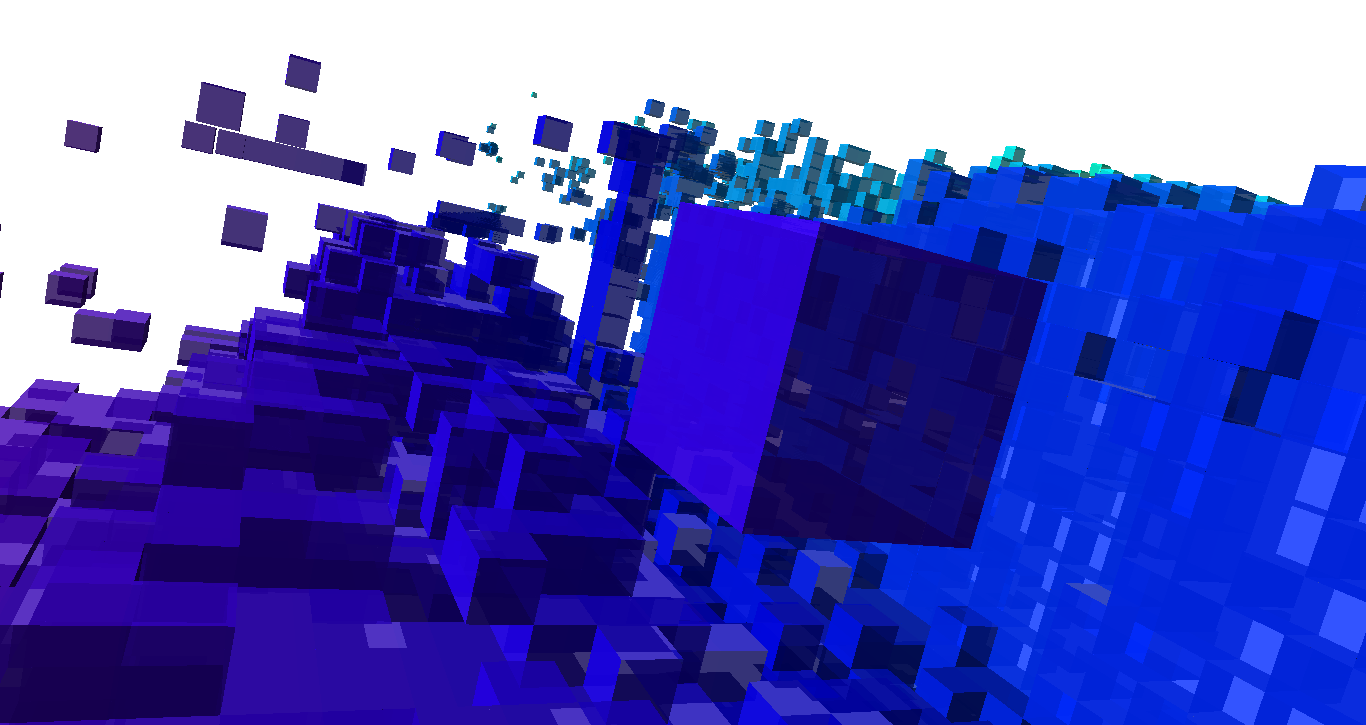
\includegraphics[width=0.9\textwidth]{img/car_and_wall1_carve2_250}  %\label{fig:}
 }
 \subfigure[Result after regularisation (graph-cut) with $\gamma = 1.8$]{
  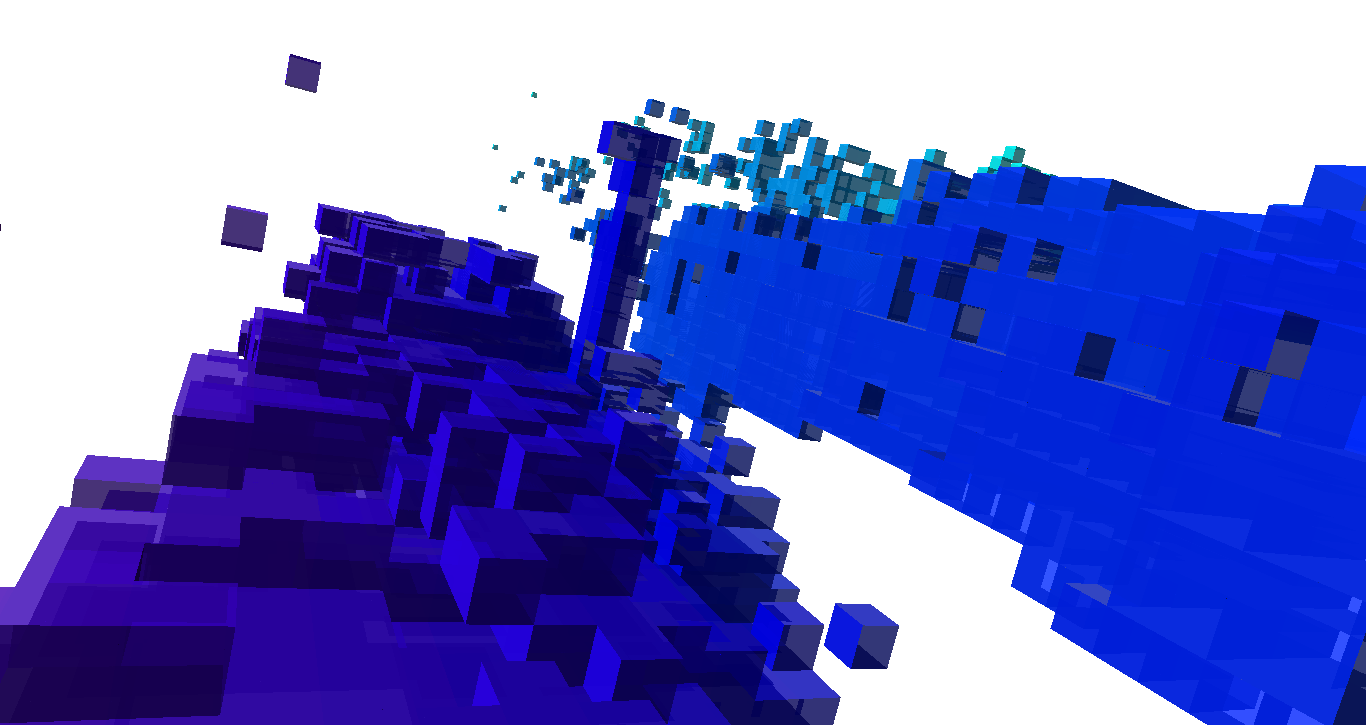
\includegraphics[width=0.9\textwidth]{img/car_and_wall1_carve2_250_gc}  %\label{fig:}
 }
 \subfigure[Result of our Visibility-Occlusion Space Carving General (Alg. \ref{alg:vis-occ-carving}) with $r=250, Pr_{incr}=Pr_{decr}=0.001$]{
  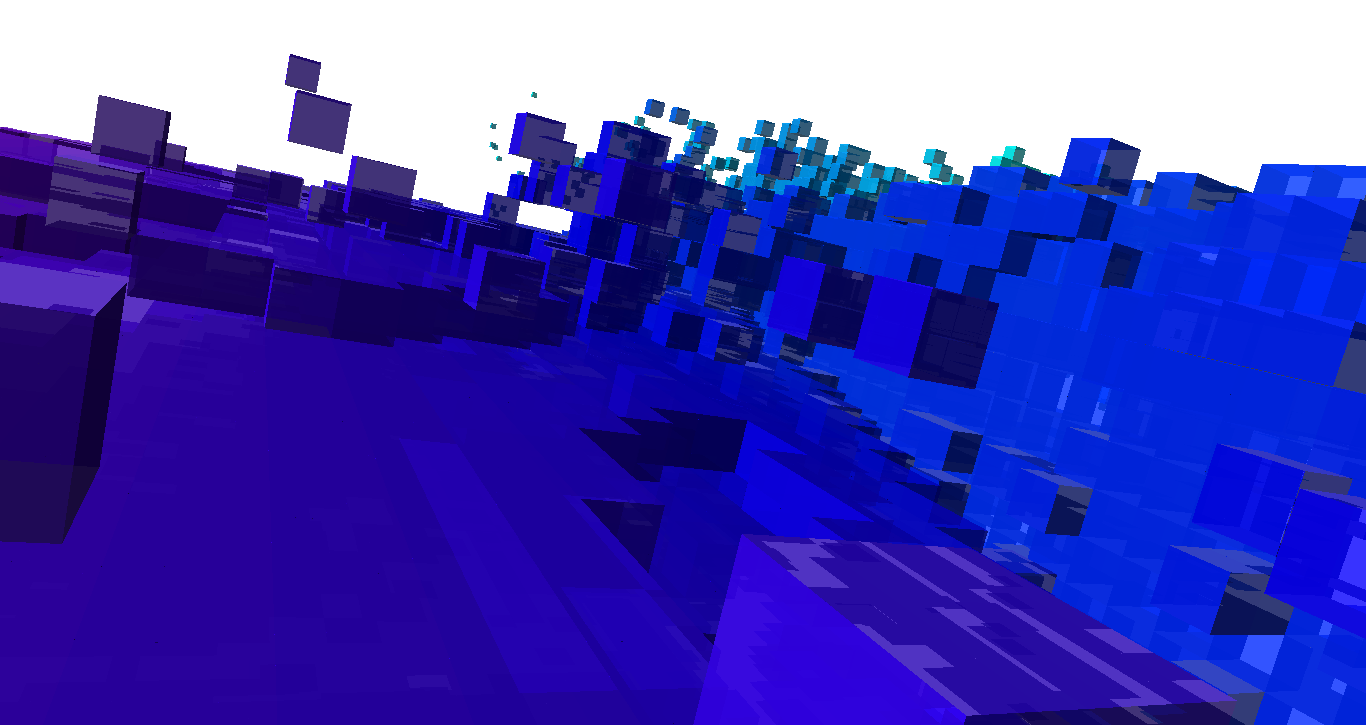
\includegraphics[width=0.9\textwidth]{img/car_and_wall1_carve3_250}  %\label{fig:}
 }
 \caption{Regularisation and extended visibility list examples car\_and\_wall1 dataset, picturing two cars and one lamppost (more details visible in Figures \ref{fig:result-typical2} and \ref{fig:result-typical2-2})}
 \label{fig:extraresults}
\end{figure}

\begin{figure}[htb!]
 \centering
 \subfigure[Example frame; notice the poor image quality]{
  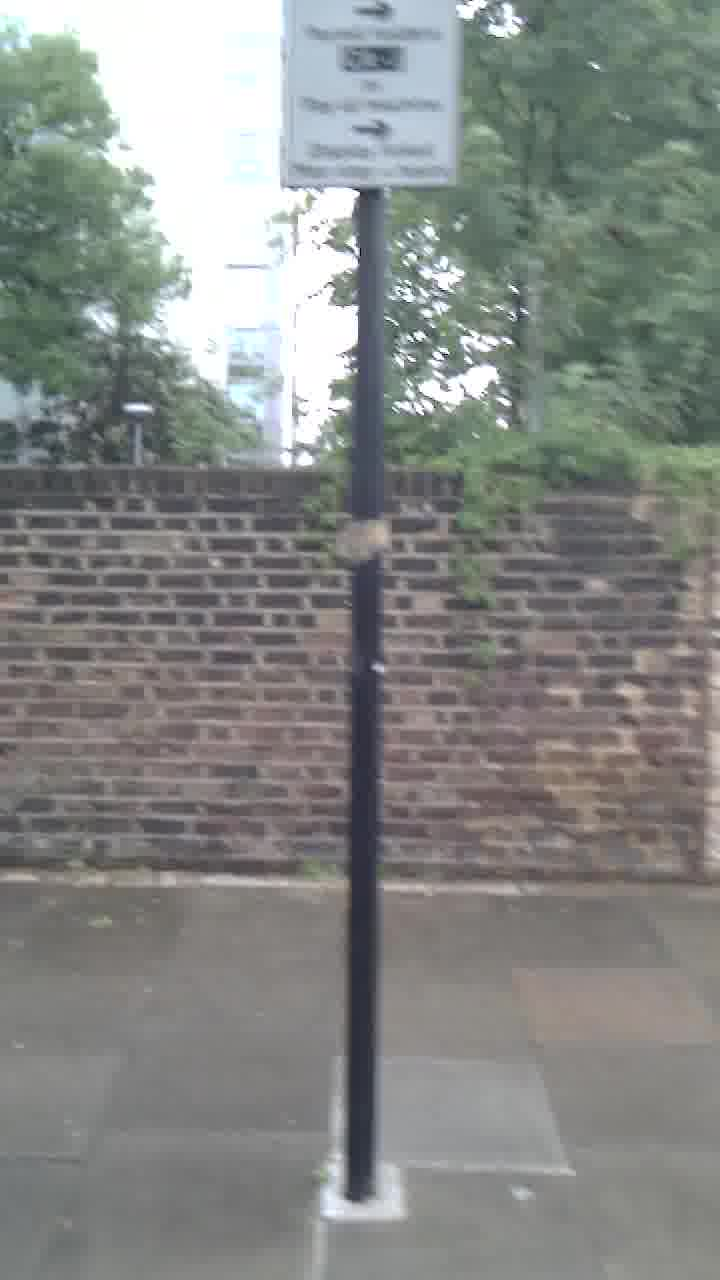
\includegraphics[width=0.3\textwidth]{img/lampposts_on_wall1_frame}  %\label{fig:}
 }
 \subfigure[Sparse point cloud and camera poses]{
  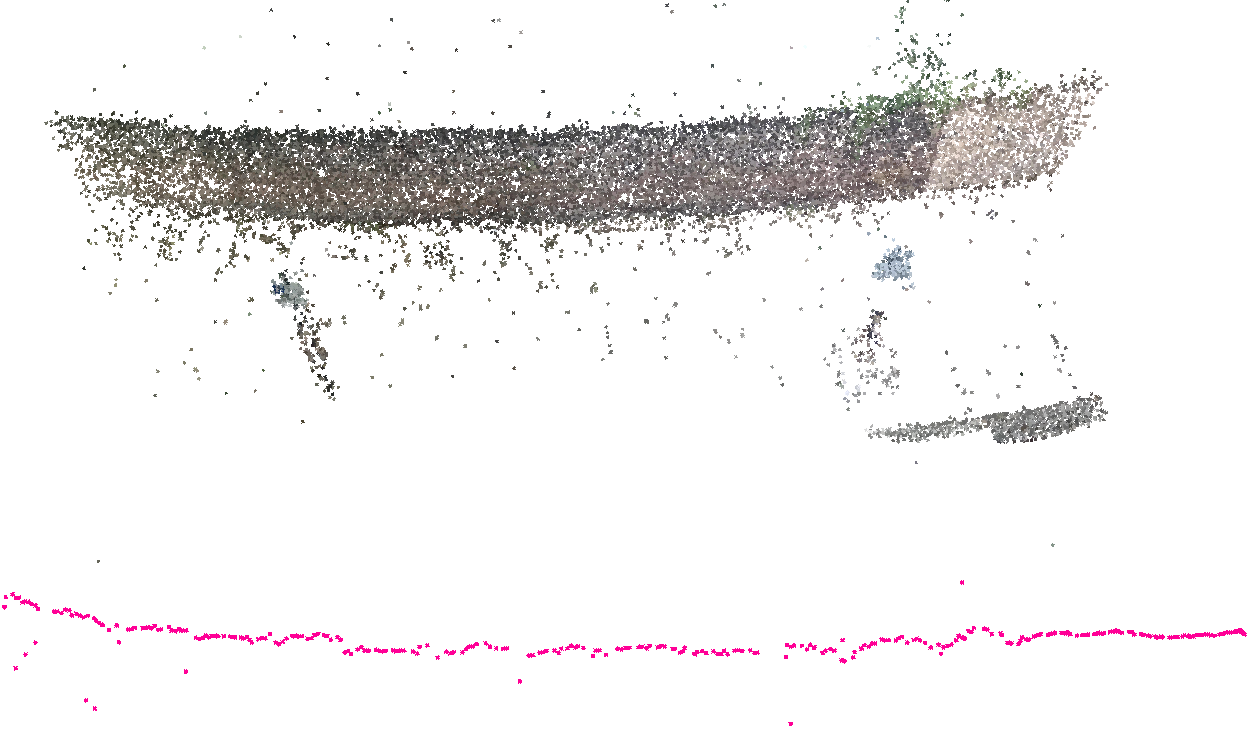
\includegraphics[width=0.65\textwidth]{img/lampposts_on_wall1_sparse}  %\label{fig:}
 }
 \subfigure[Discretised sparse point cloud ($r=1000$)]{
  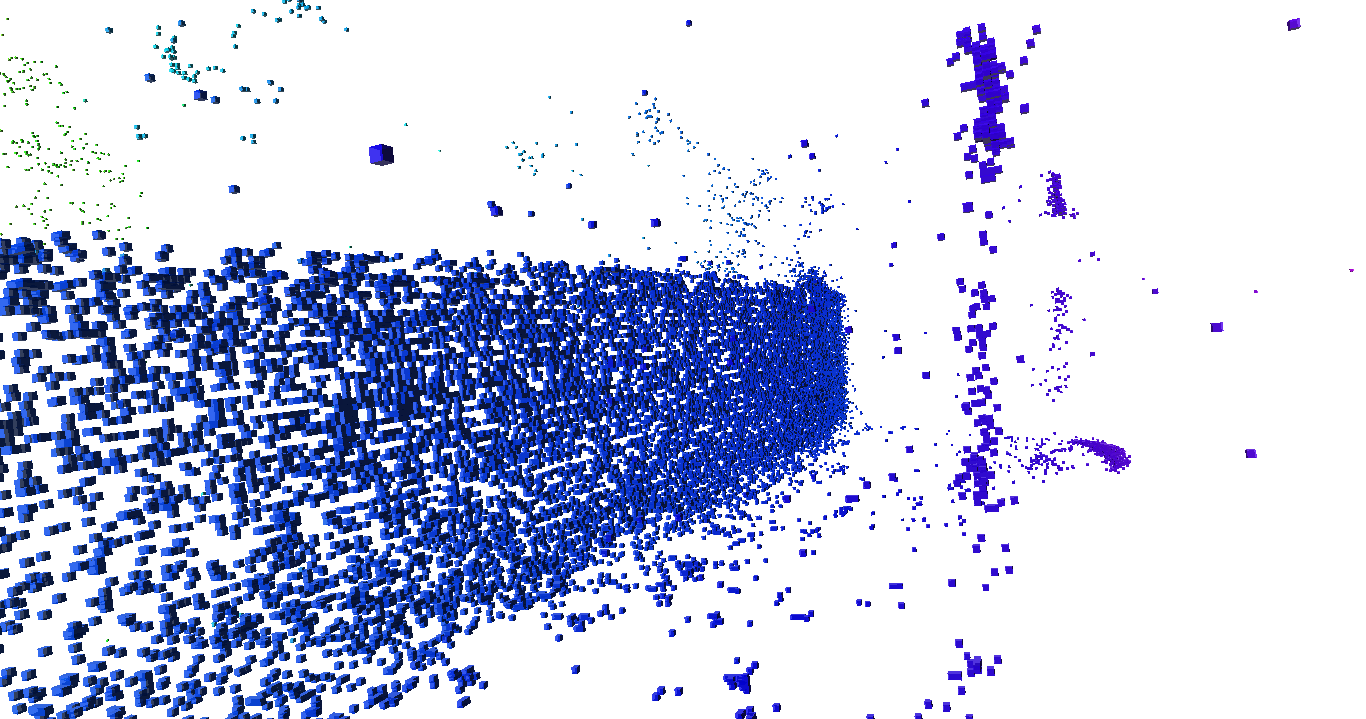
\includegraphics[width=1\textwidth]{img/lampposts_on_wall1_carve0}  %\label{fig:}
 }
 \caption{Typical result 2: lampposts\_on\_wall1 dataset}
 \label{fig:result-typical1}
\end{figure}
\begin{figure}[htb!]
 \centering
 \subfigure[Result of our Visibility Space Carving (Alg. \ref{alg:vis-carving}) with $r=500$; Notice the occupied-labelled space above and underneath the carved space, caused by an insufficient amount of feature points in the trees above the wall and on the ground.]{
  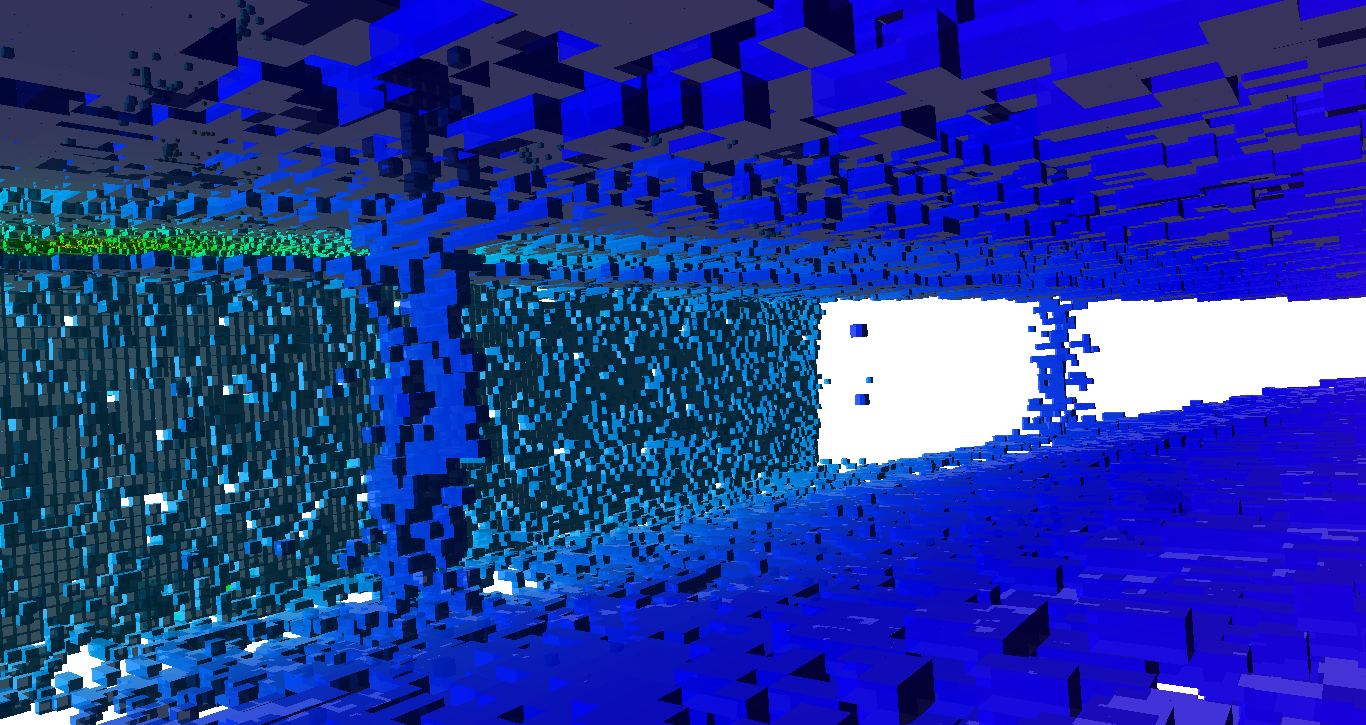
\includegraphics[width=0.95\textwidth]{img/lampposts_on_wall1_carve1}  %\label{fig:}
 }
 \subfigure[Result of our Visibility-Occlusion Space Carving Veto (Alg. \ref{alg:vis-occ-carving-veto}) with $r=1000, Pr_{incr}=0.005$]{
  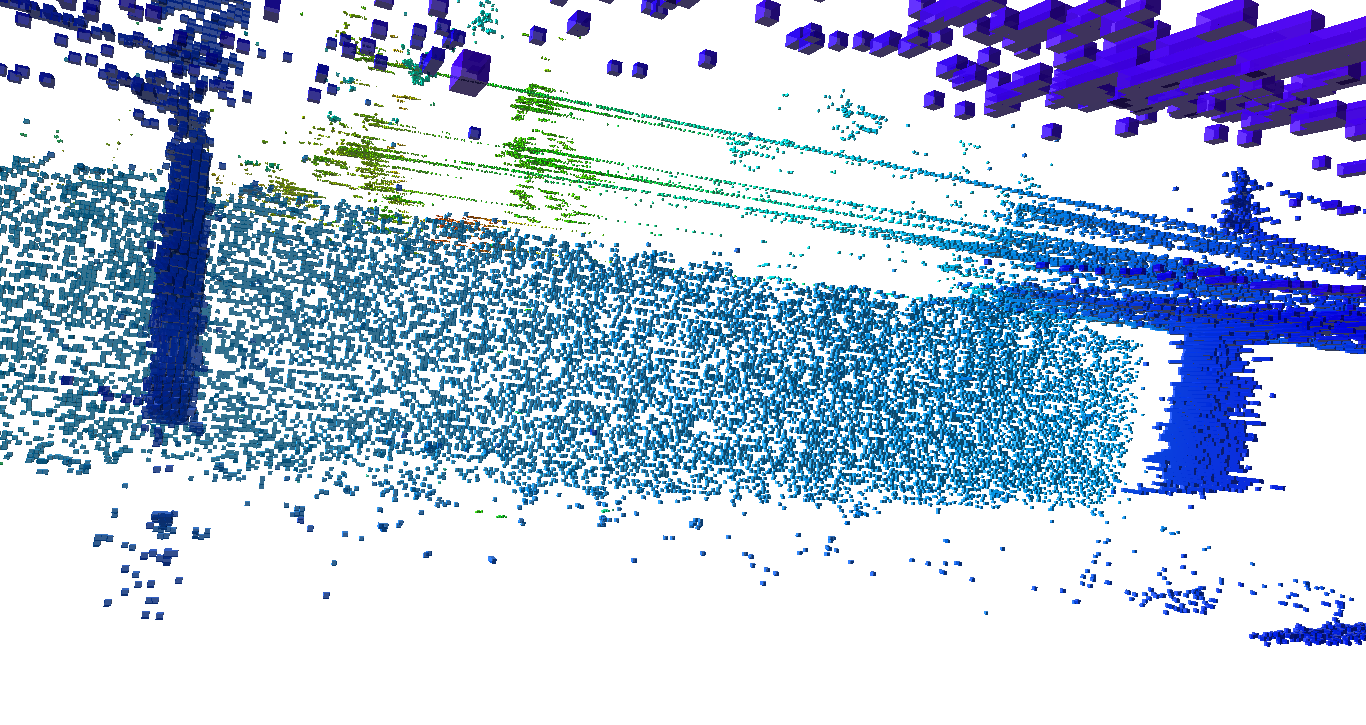
\includegraphics[width=0.95\textwidth]{img/lampposts_on_wall1_carve2}  %\label{fig:}
 }
 \subfigure[Result of CMVS/PMVS \cite{Furukawa2010}]{
  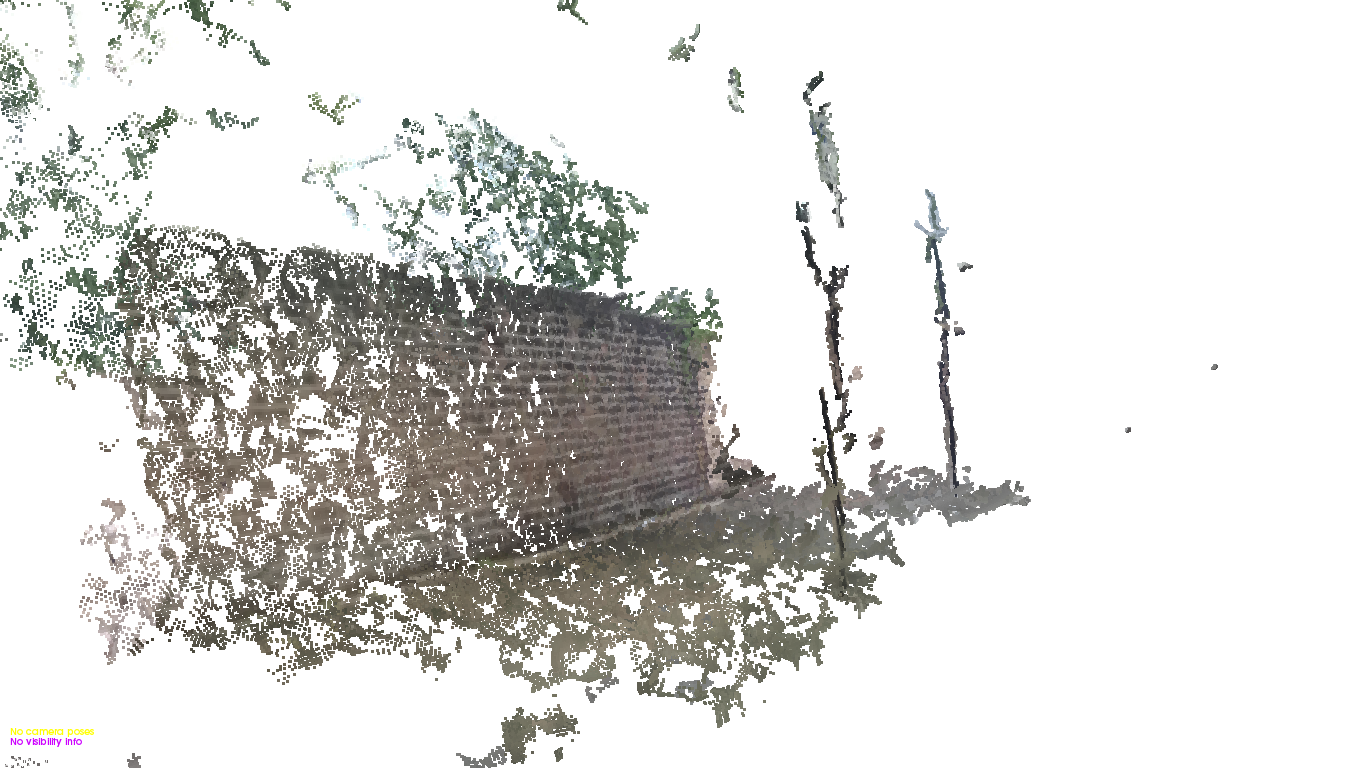
\includegraphics[width=0.95\textwidth]{img/lampposts_on_wall1_dense}  %\label{fig:}
 }
 \caption{Typical result 2: lampposts\_on\_wall1 dataset (cont.)}
 \label{fig:result-typical1-2}
\end{figure}

\begin{figure}[htb!]
 \centering
 \subfigure[Example frame]{
  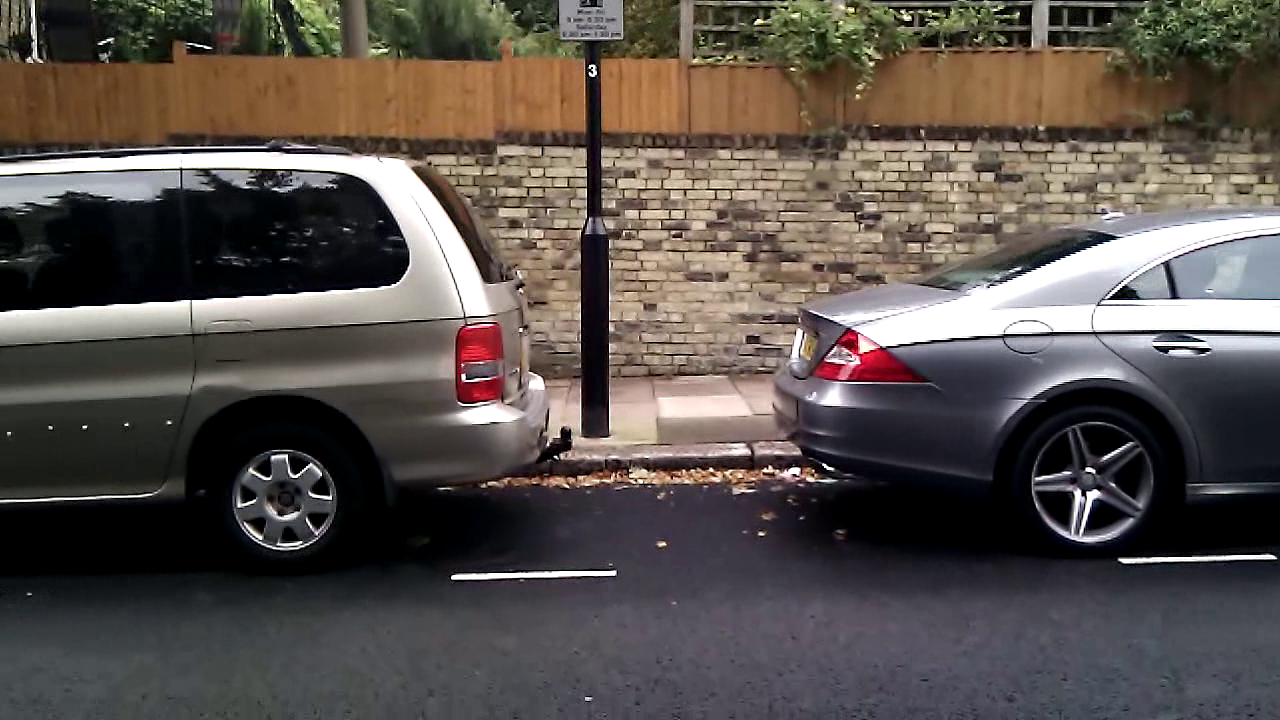
\includegraphics[width=0.9\textwidth]{img/car_and_wall1_frame}  %\label{fig:}
 }
 \subfigure[Sparse point cloud and camera poses, annotated with visibility lines from one point (hinting at possible occluding object locations)]{
  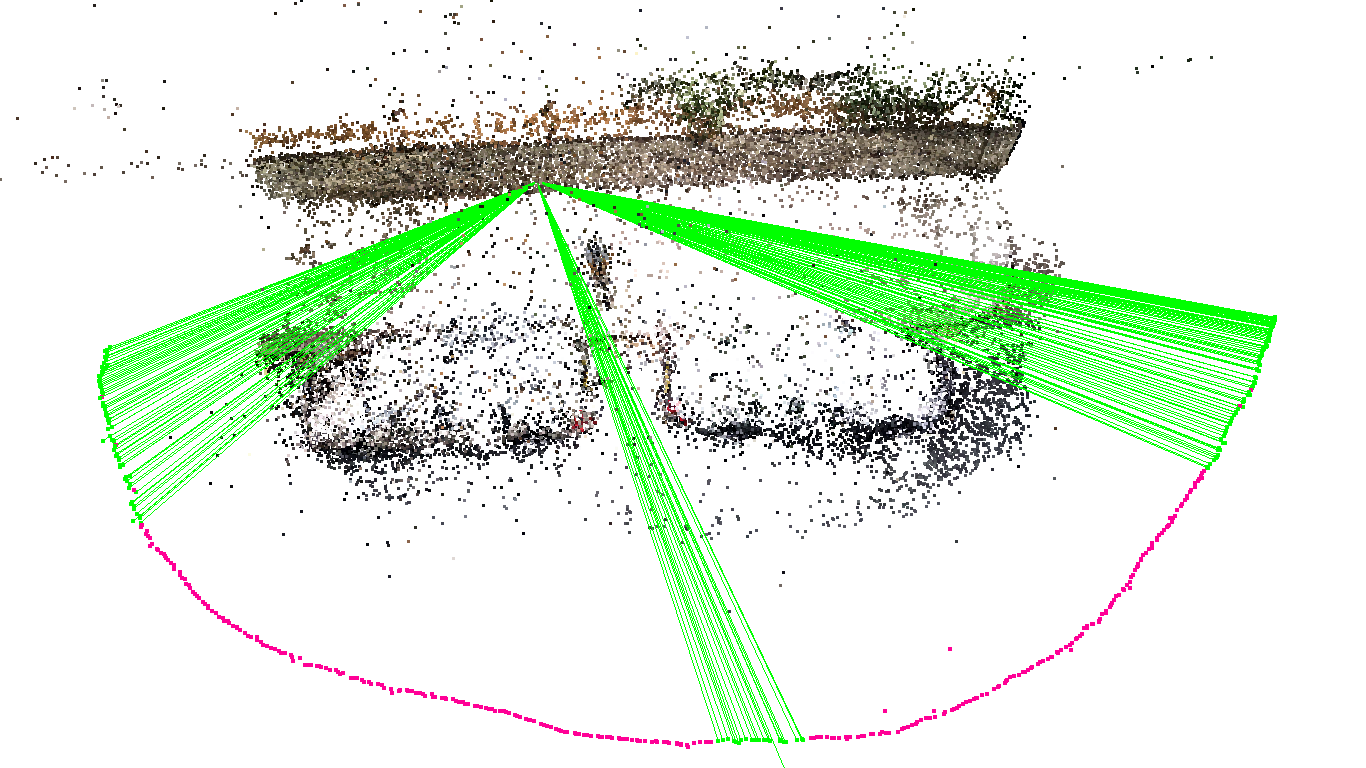
\includegraphics[width=1\textwidth]{img/car_and_wall1_sparse}  %\label{fig:}
 }
 \subfigure[Discretised sparse point cloud ($r=1000$)]{
  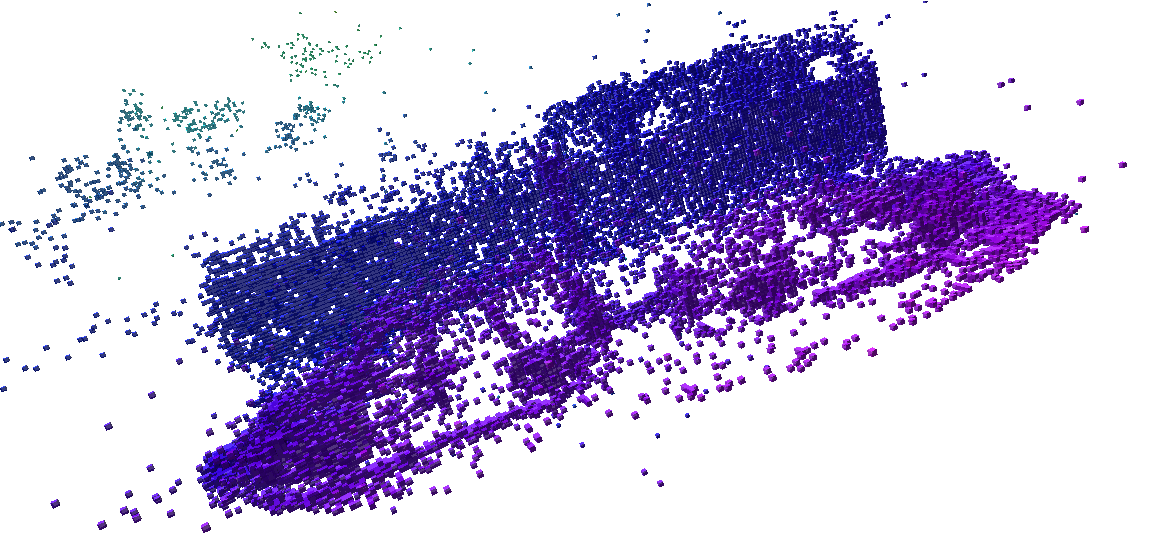
\includegraphics[width=1\textwidth]{img/car_and_wall1_carve0}  %\label{fig:}
 }
 \caption{Typical result 2: car\_and\_wall1 dataset}
 \label{fig:result-typical2}
\end{figure}
\begin{figure}[htb!]
 \centering
 \subfigure[Result of our Visibility Space Carving (Alg. \ref{alg:vis-carving}) with $r=1000$; Incorrectly occupied-labelled space inside the red `box', caused by an insufficient amount of feature points above the wall (\eg on trees), was removed for visualisation purposes.]{
  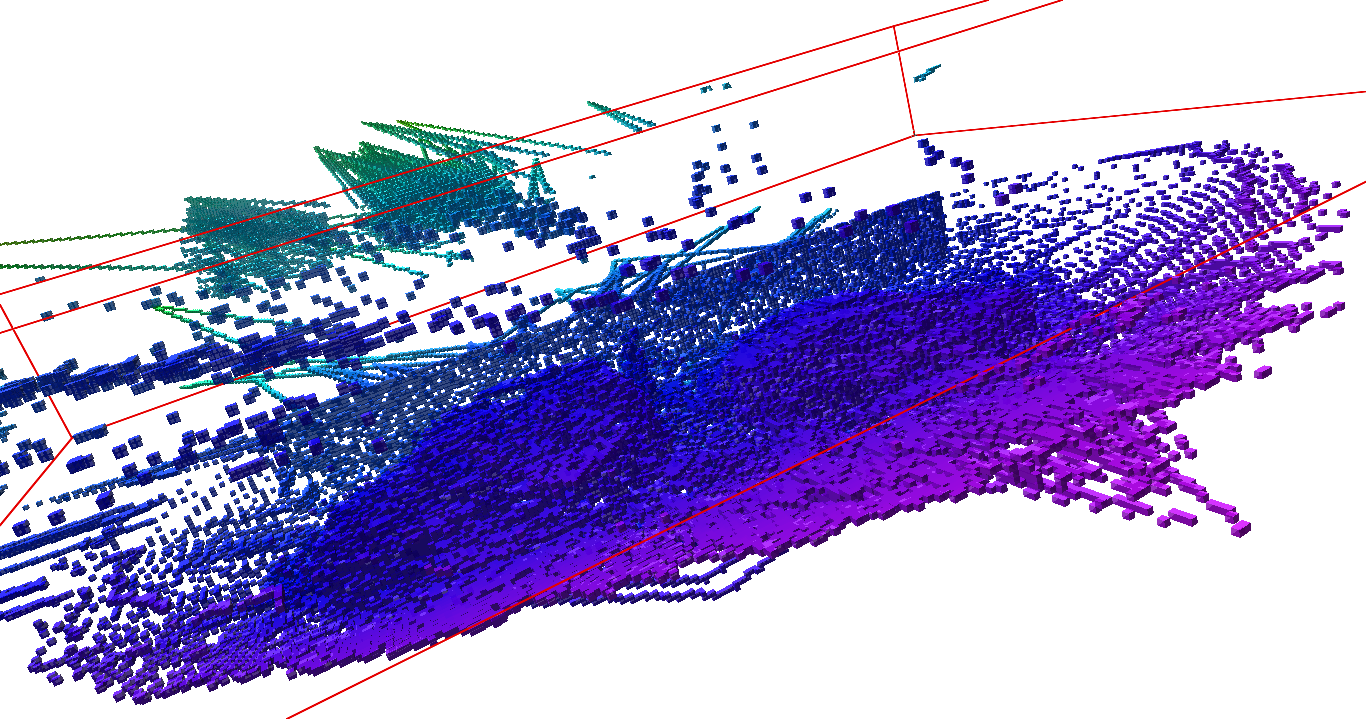
\includegraphics[width=1\textwidth]{img/car_and_wall1_carve1}  %\label{fig:}
 }
 \subfigure[Result of our Visibility-Occlusion Space Carving Veto (Alg. \ref{alg:vis-occ-carving-veto}) with $r=2500, Pr_{incr}=0.005$]{
  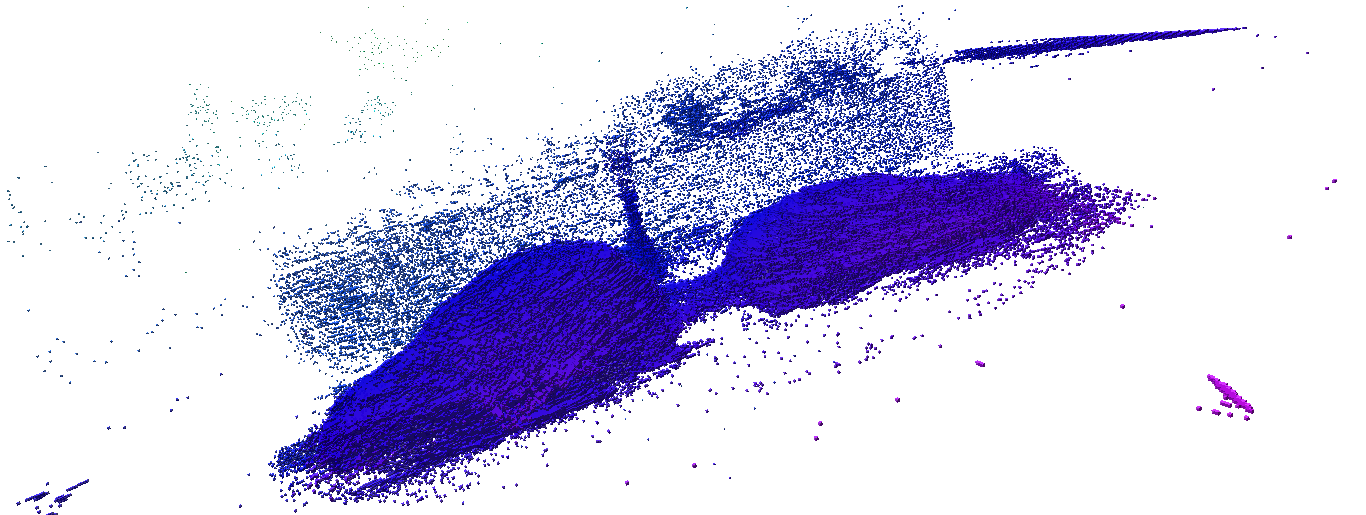
\includegraphics[width=1\textwidth]{img/car_and_wall1_carve2}  %\label{fig:}
 }
 \subfigure[Result of CMVS/PMVS \cite{Furukawa2010}]{
  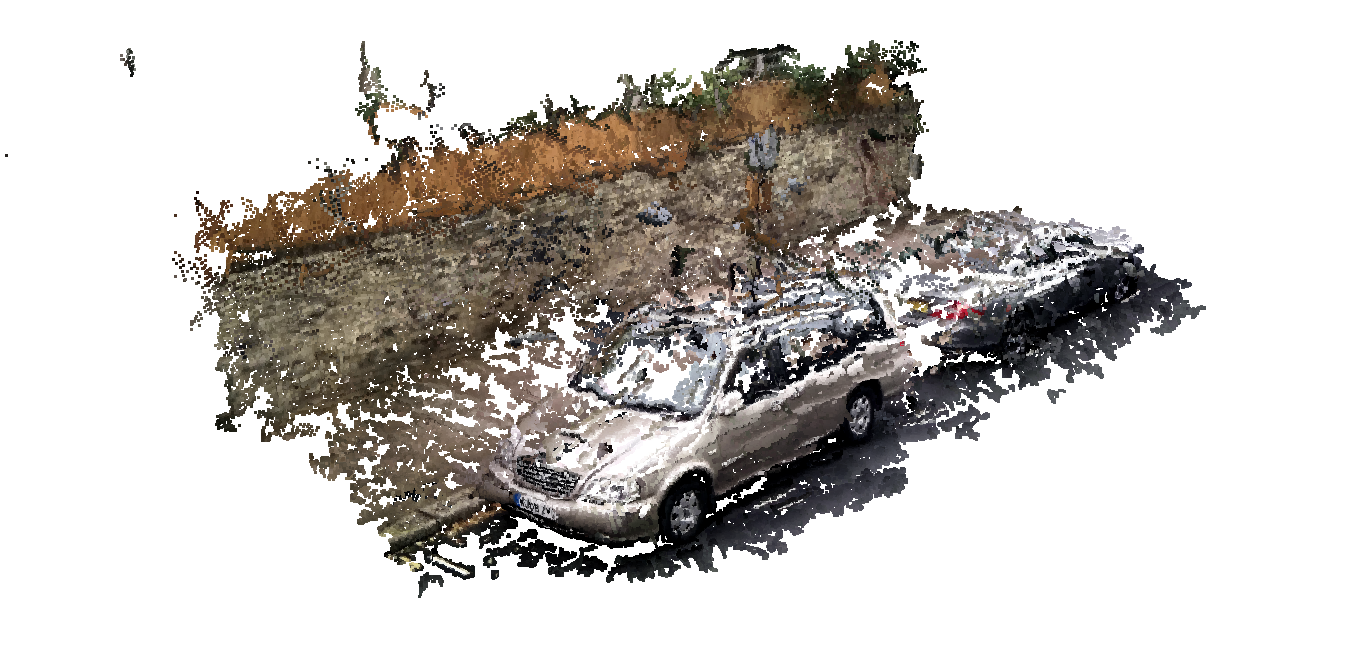
\includegraphics[width=1\textwidth]{img/car_and_wall1_dense}  %\label{fig:}
 }
 \caption{Typical result 2: car\_and\_wall1 dataset (cont.)}
 \label{fig:result-typical2-2}
\end{figure}



\begin{figure}[htb!]
 \centering
 \subfigure[Example frame]{
  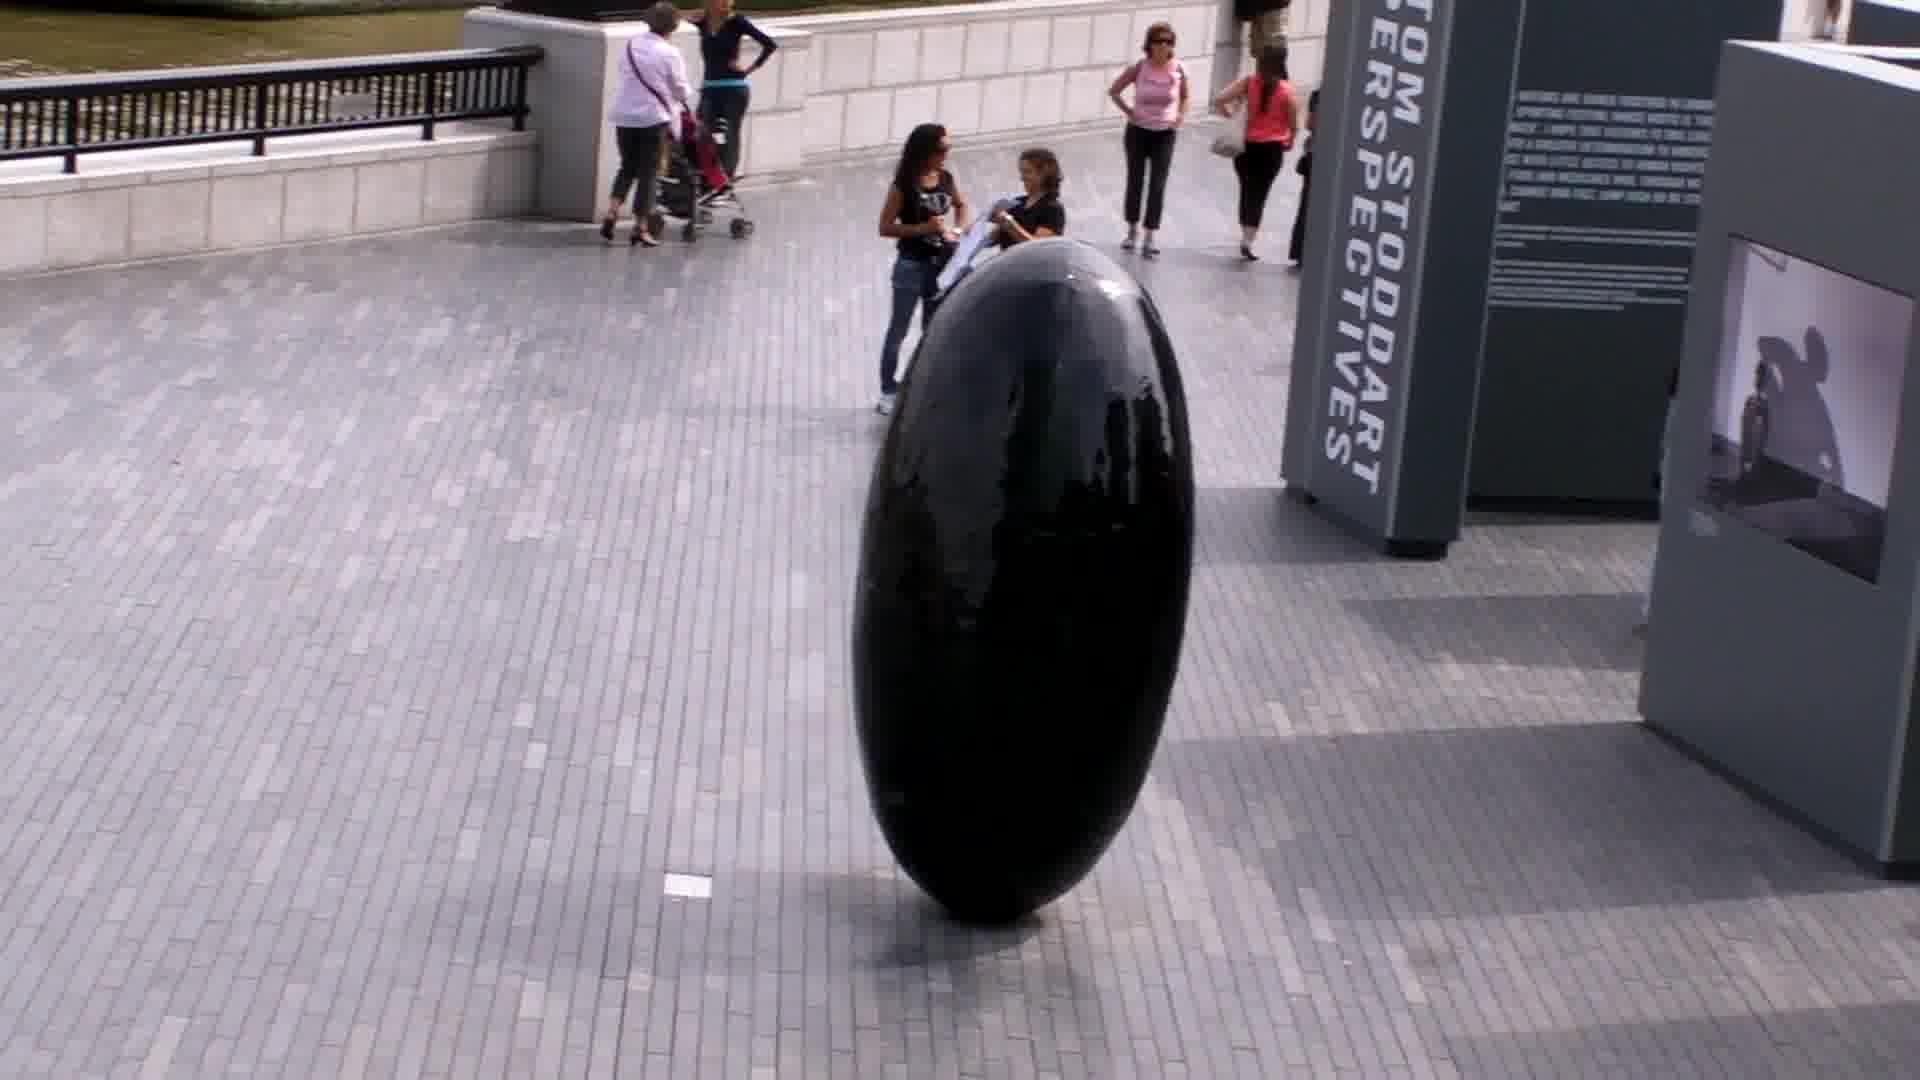
\includegraphics[width=0.9\textwidth]{img/sculpture1_frame}  %\label{fig:}
 }
 \subfigure[Sparse point cloud and camera poses, annotated with visibility lines from one point]{
  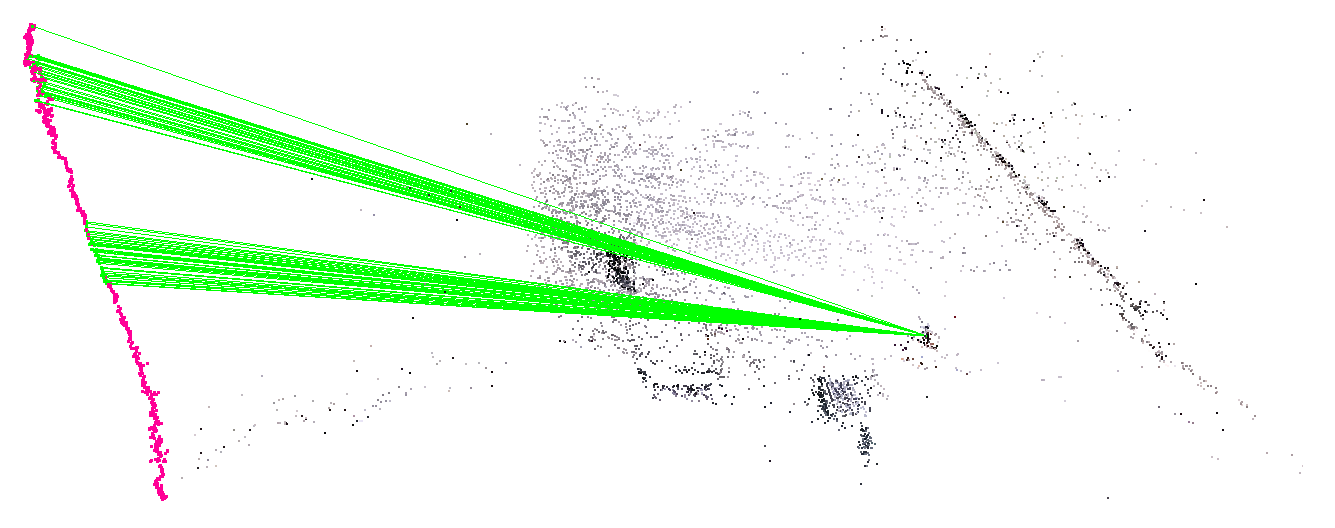
\includegraphics[width=0.9\textwidth]{img/sculpture1_sparse}  %\label{fig:}
 }
 \subfigure[Discretised sparse point cloud ($r=1000$)]{
  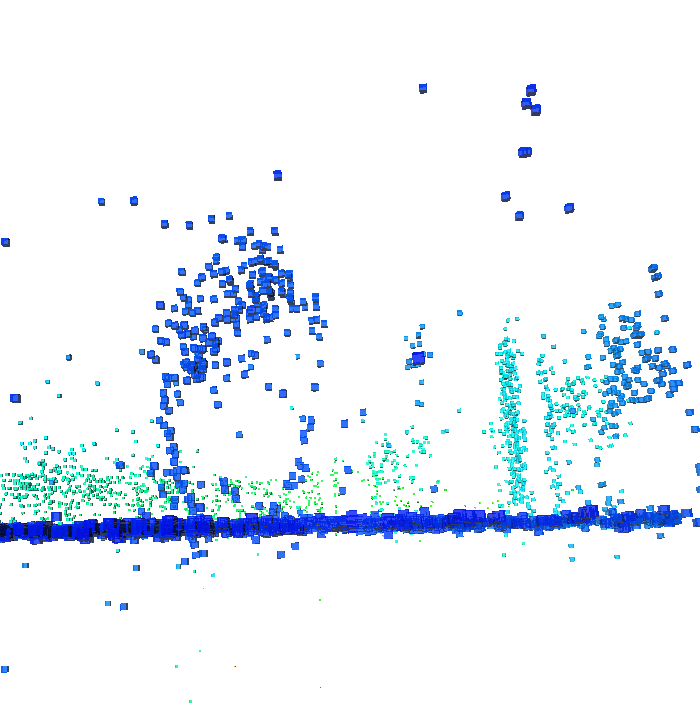
\includegraphics[width=0.45\textwidth]{img/sculpture1_carve0}  \label{fig:sculpture1_carve0}
 }
 \subfigure[Discretised sparse point cloud ($r=1000$), carveviewer; notice the incorrectly visible ground voxels (blue-ish) on the lower half of the sculpture]{
  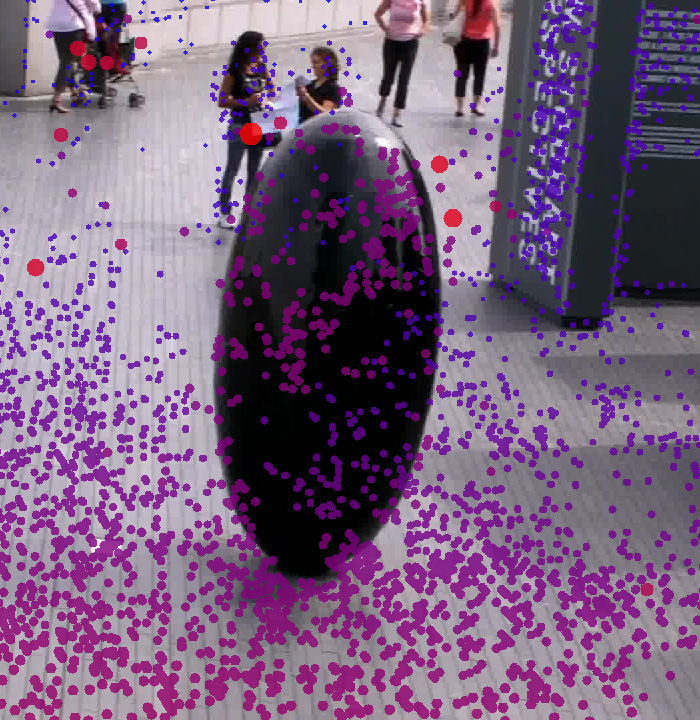
\includegraphics[width=0.45\textwidth]{img/sculpture1_carve0_ann}  %\label{fig:}
 }
 \caption{Good result 2: memorial dataset}
 \label{fig:result-good1}
\end{figure}
\begin{figure}[htb!]
 \centering
 \subfigure[Result of our Visibility Space Carving (Alg. \ref{alg:vis-carving}) with $r=250$]{
  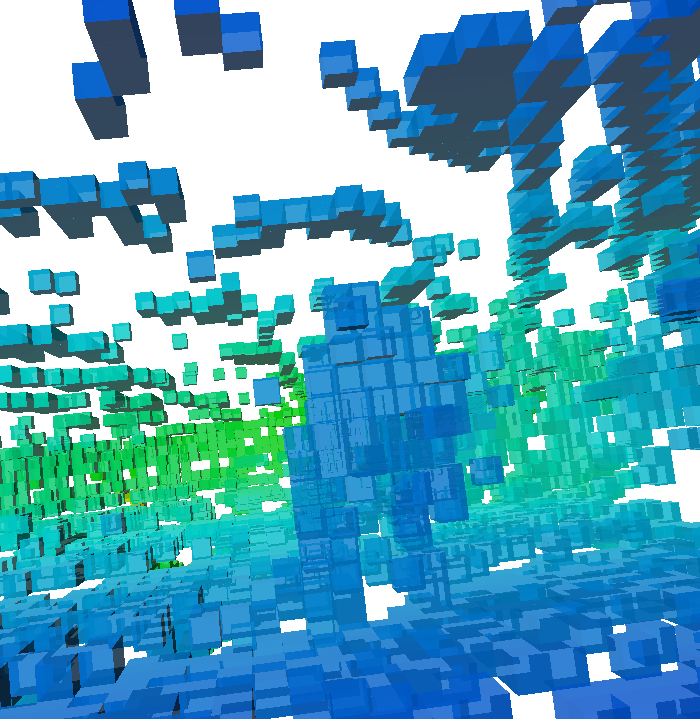
\includegraphics[width=0.45\textwidth]{img/sculpture1_carve1}  %\label{fig:}
 }
 \subfigure[Result of our Visibility Space Carving (Alg. \ref{alg:vis-carving}) with $r=250$, carveviewer]{
  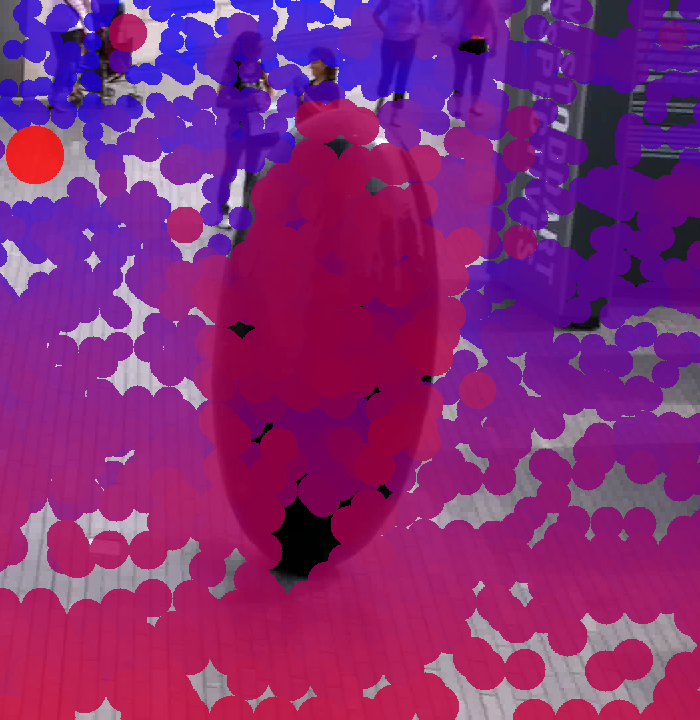
\includegraphics[width=0.45\textwidth]{img/sculpture1_carve1_ann}  %\label{fig:}
 }
 \subfigure[Result of our Visibility-Occlusion Space Carving Veto (Alg. \ref{alg:vis-occ-carving-veto}) with $r=1000, Pr_{incr}=0.001$]{
  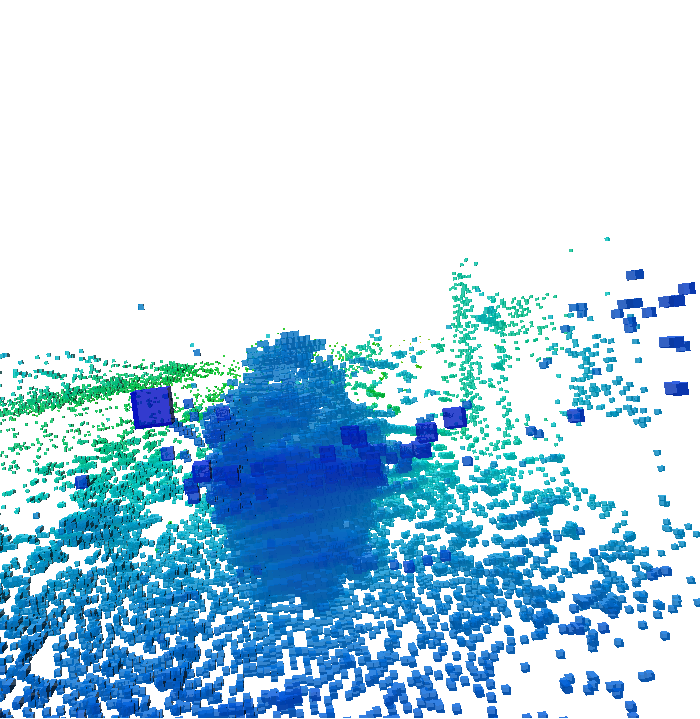
\includegraphics[width=0.45\textwidth]{img/sculpture1_carve2}  %\label{fig:}
 }
 \subfigure[Result of our Visibility-Occlusion Space Carving Veto (Alg. \ref{alg:vis-occ-carving-veto}) with $r=1000, Pr_{incr}=0.001$, carveviewer]{
  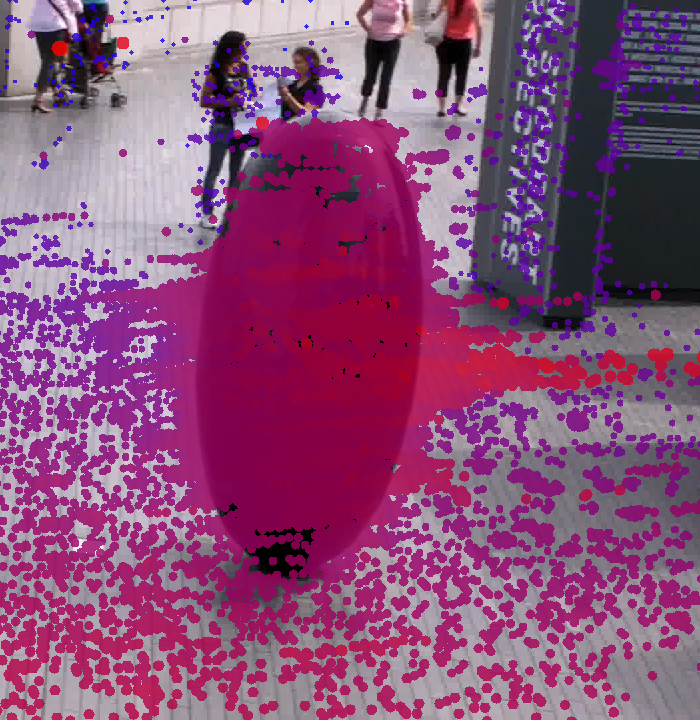
\includegraphics[width=0.45\textwidth]{img/sculpture1_carve2_ann}  %\label{fig:}
 }
 \subfigure[Result of CMVS/PMVS \cite{Furukawa2010}. Notice the similarity with the sparse point cloud as seen from this angle, shown in \ref{fig:sculpture1_carve0}; lack of texture clearly influences both sparse and dense point cloud reconstructions.]{
  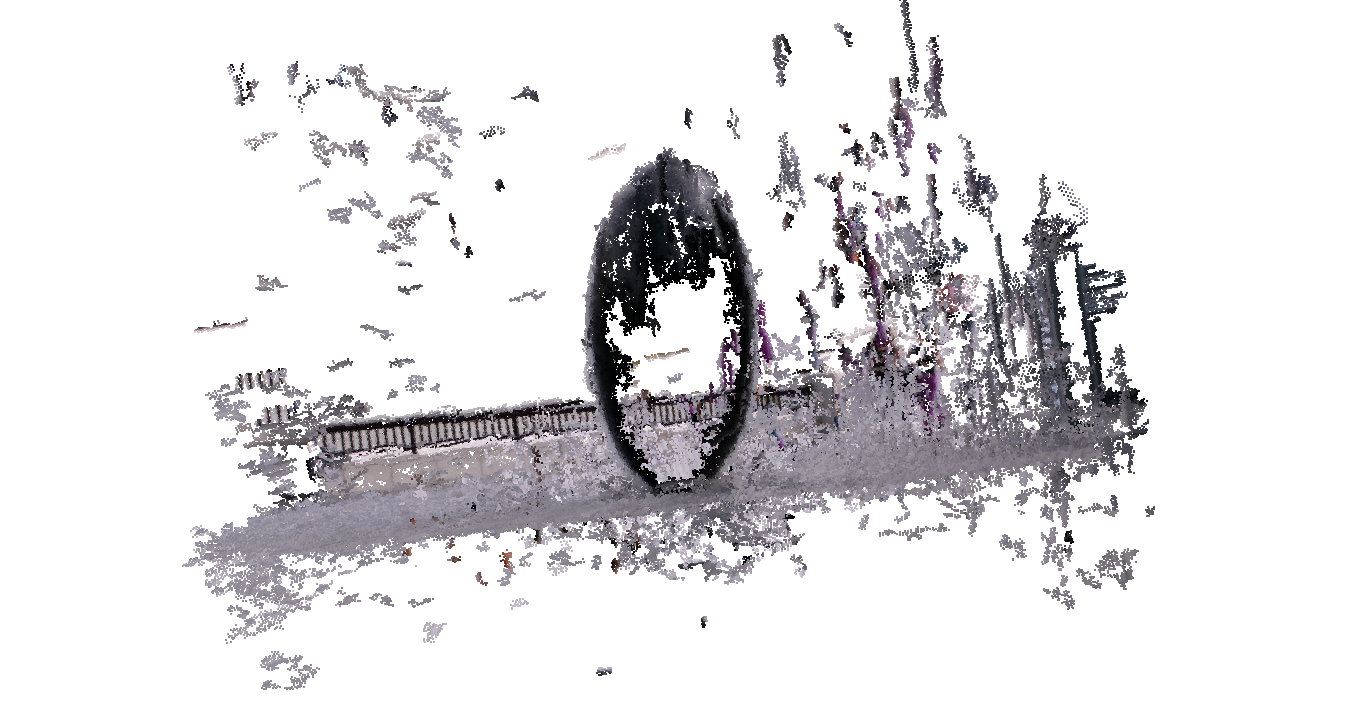
\includegraphics[width=0.90\textwidth]{img/sculpture1_dense}  %\label{fig:}
 }
 %\subfigure[Result of CMVS/PMVS \cite{Furukawa2010}, carveviewer]{
 % 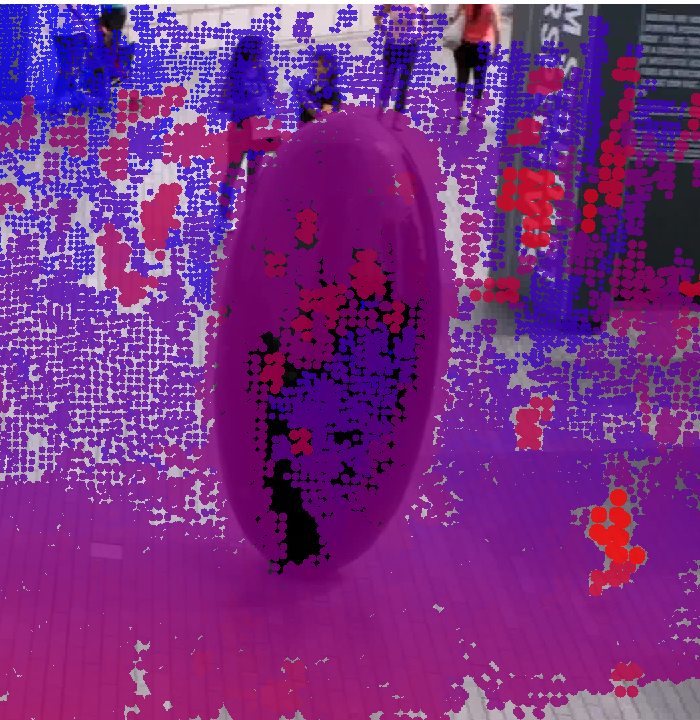
\includegraphics[width=0.45\textwidth]{img/sculpture1_dense_ann}  %\label{fig:}
 %}
 \caption{Good result 1: sculpture1 dataset (cont.)}
 \label{fig:result-good1-2}
\end{figure}


\begin{figure}[htb!]
 \centering
 \subfigure[Example frame]{
  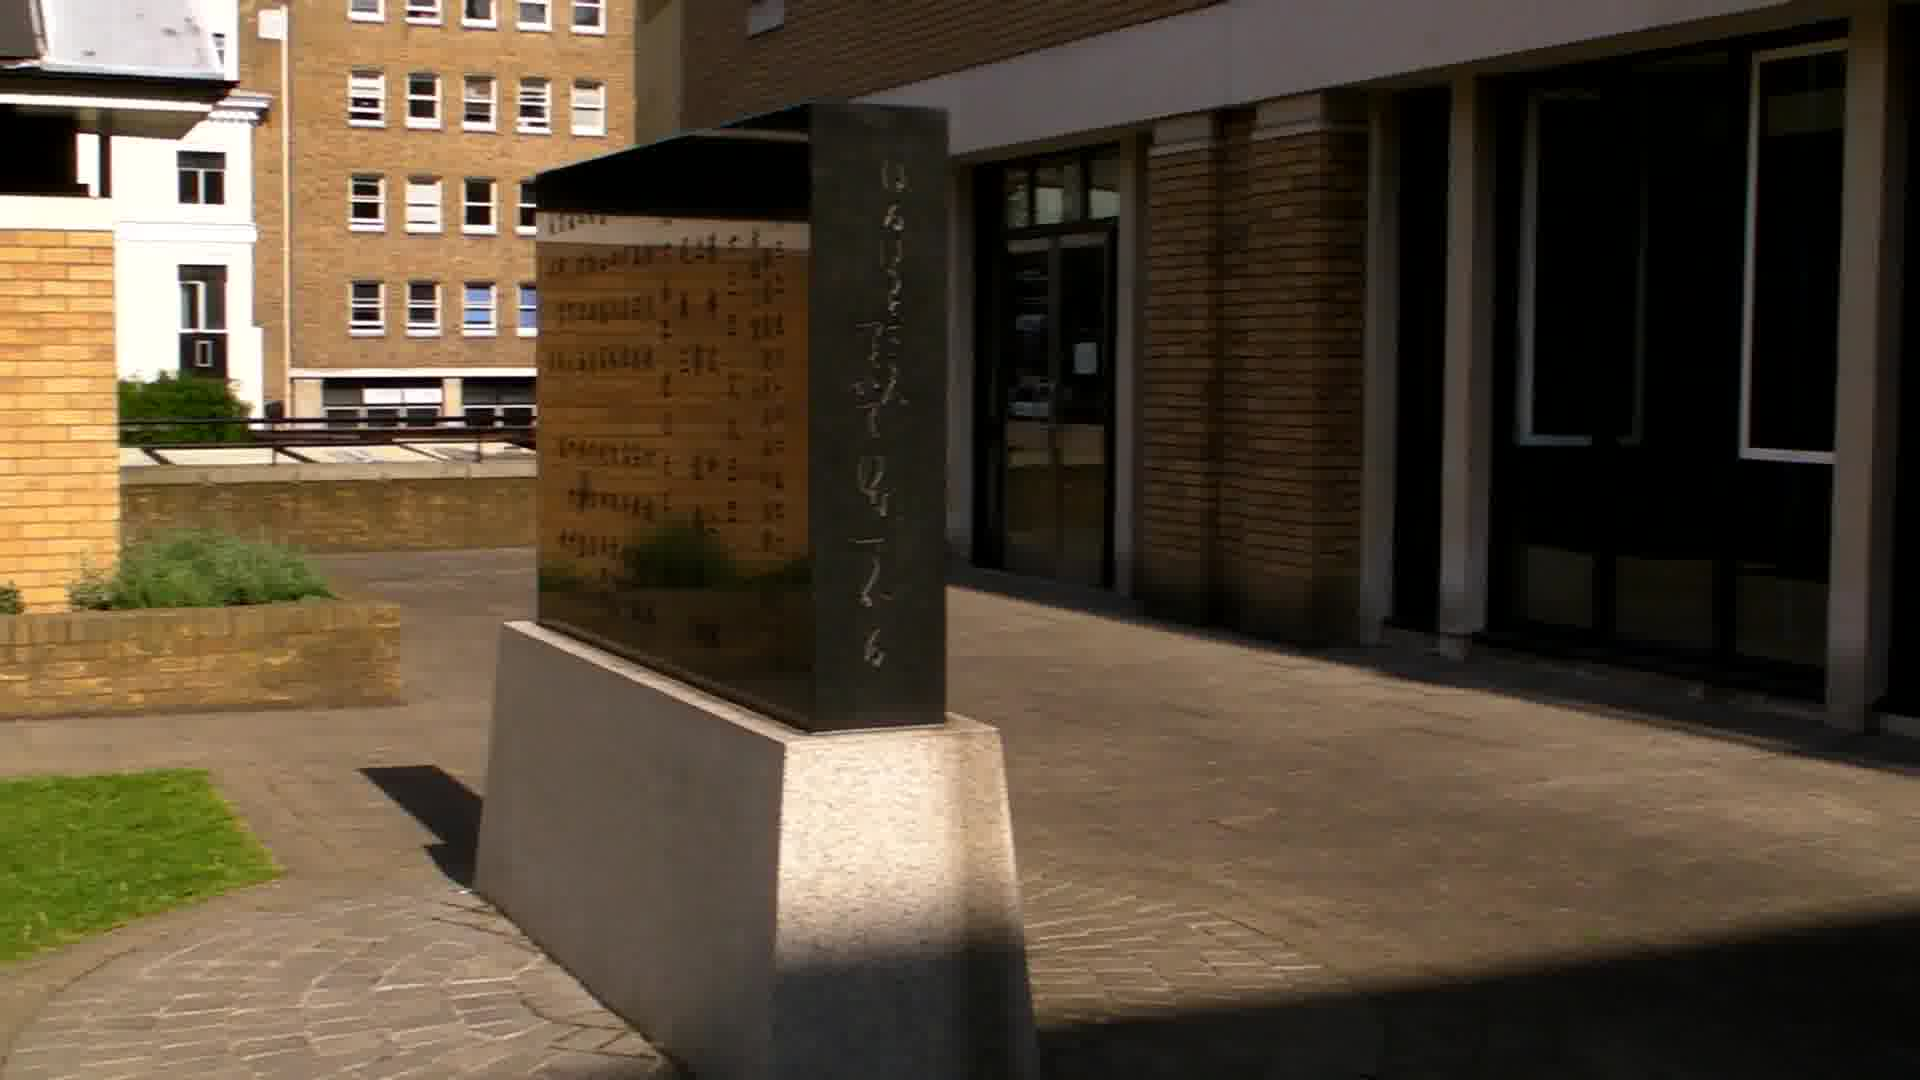
\includegraphics[width=0.9\textwidth]{img/memorial_frame}  %\label{fig:}
 }
 \subfigure[Sparse point cloud and camera poses]{
  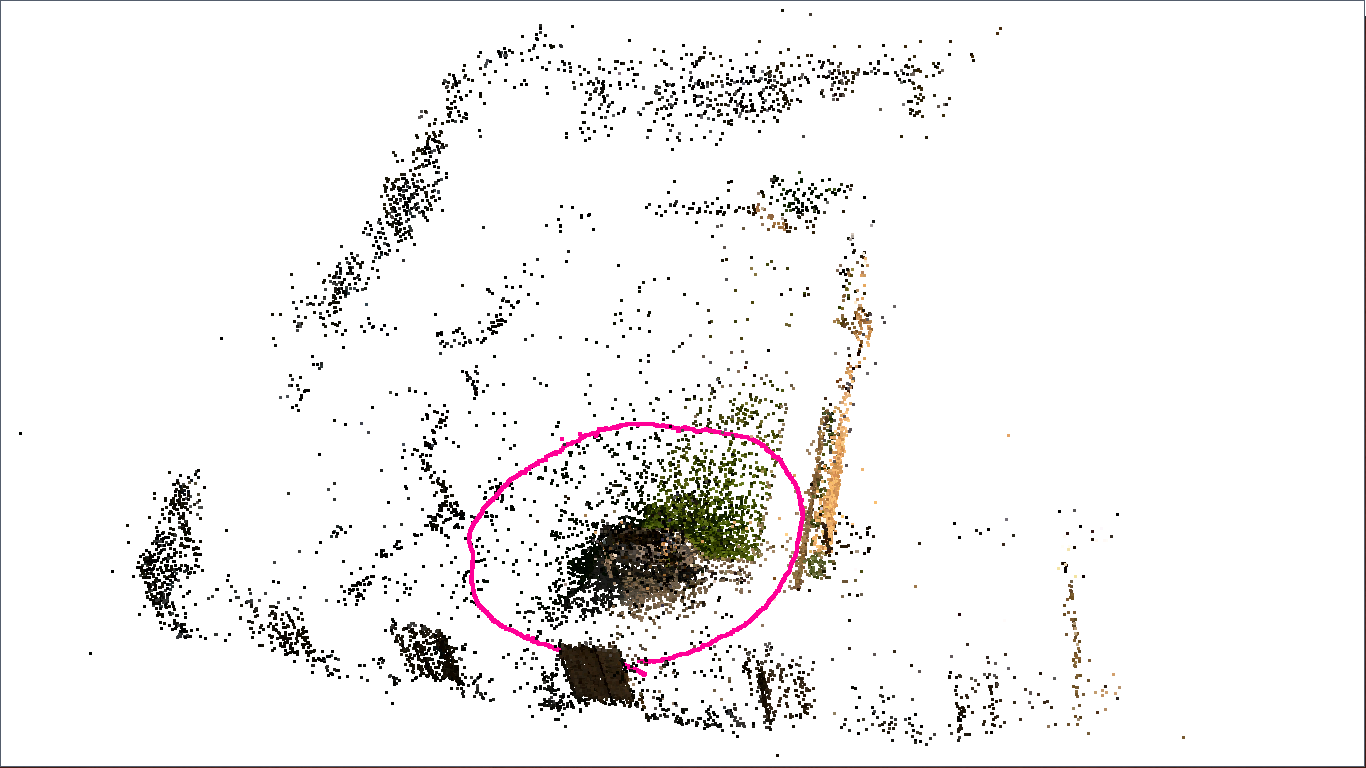
\includegraphics[width=0.9\textwidth]{img/memorial_sparse}  %\label{fig:}
 }
 \subfigure[Discretised sparse point cloud ($r=2500$)]{
  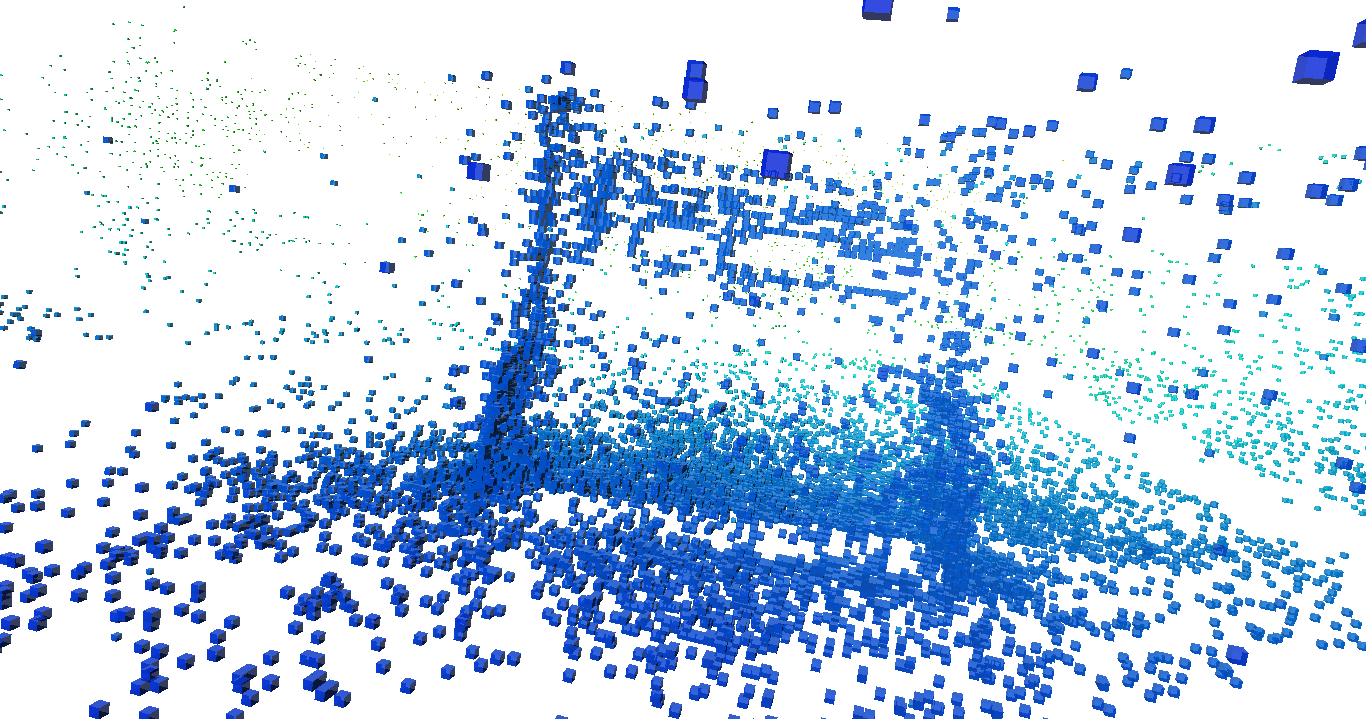
\includegraphics[width=0.9\textwidth]{img/memorial_carve0}  \label{fig:memorial_carve0}
 }
 \caption{Good result 2: memorial dataset}
 \label{fig:result-good2}
\end{figure}
\begin{figure}[htb!]
 \centering
 \subfigure[Result of our Visibility Space Carving (Alg. \ref{alg:vis-carving}) with $r=500$]{
  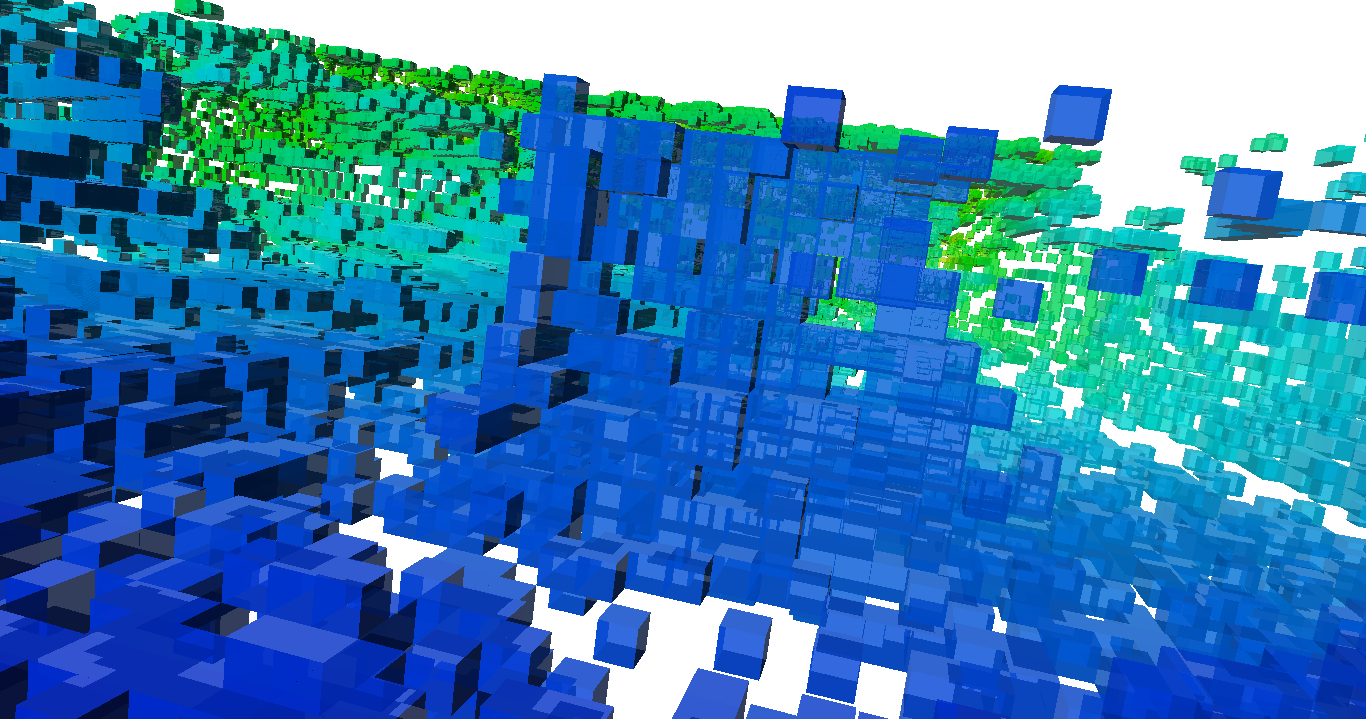
\includegraphics[width=0.9\textwidth]{img/memorial_carve1}  %\label{fig:}
 }
 \subfigure[Result of our Visibility-Occlusion Space Carving Veto (Alg. \ref{alg:vis-occ-carving-veto}) with $r=2500, Pr_{incr}=0.001$; Top-left: scene overview]{
  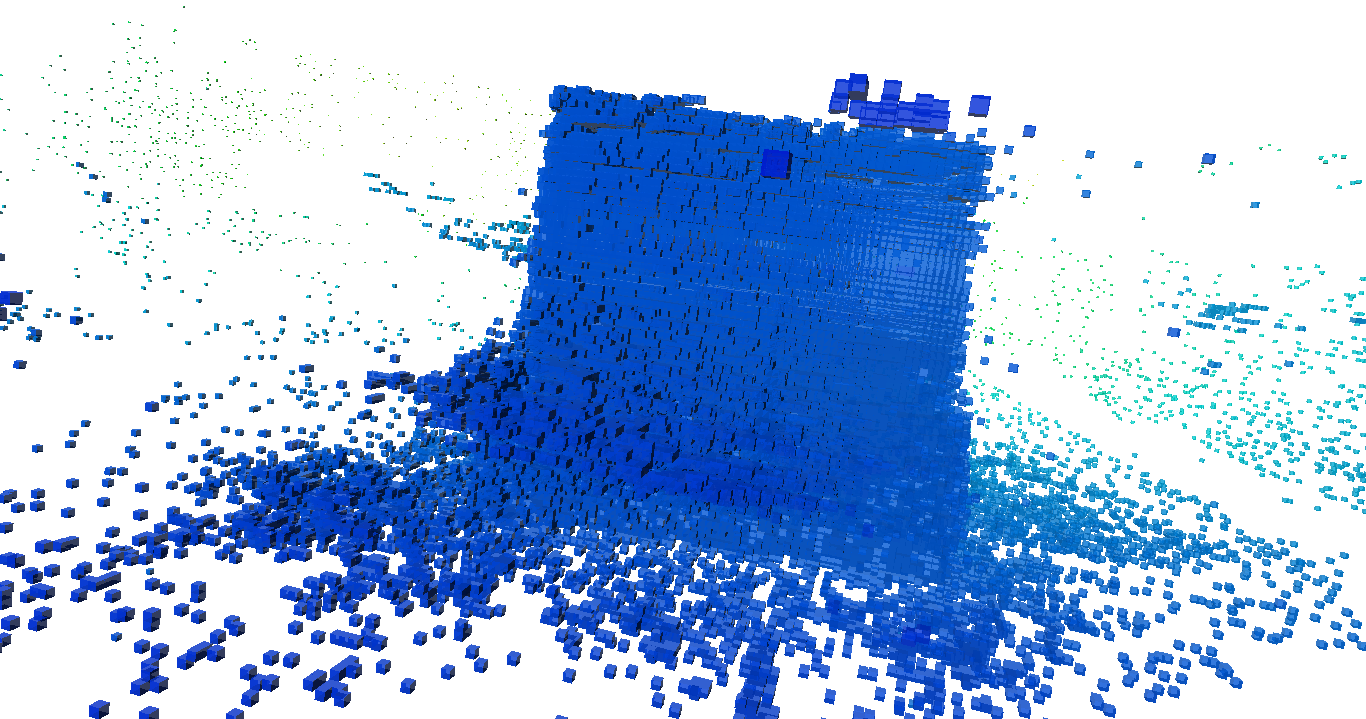
\includegraphics[width=0.9\textwidth]{img/memorial_carve2}  %\label{fig:}
 }
 \subfigure[Result of CMVS/PMVS \cite{Furukawa2010}]{
  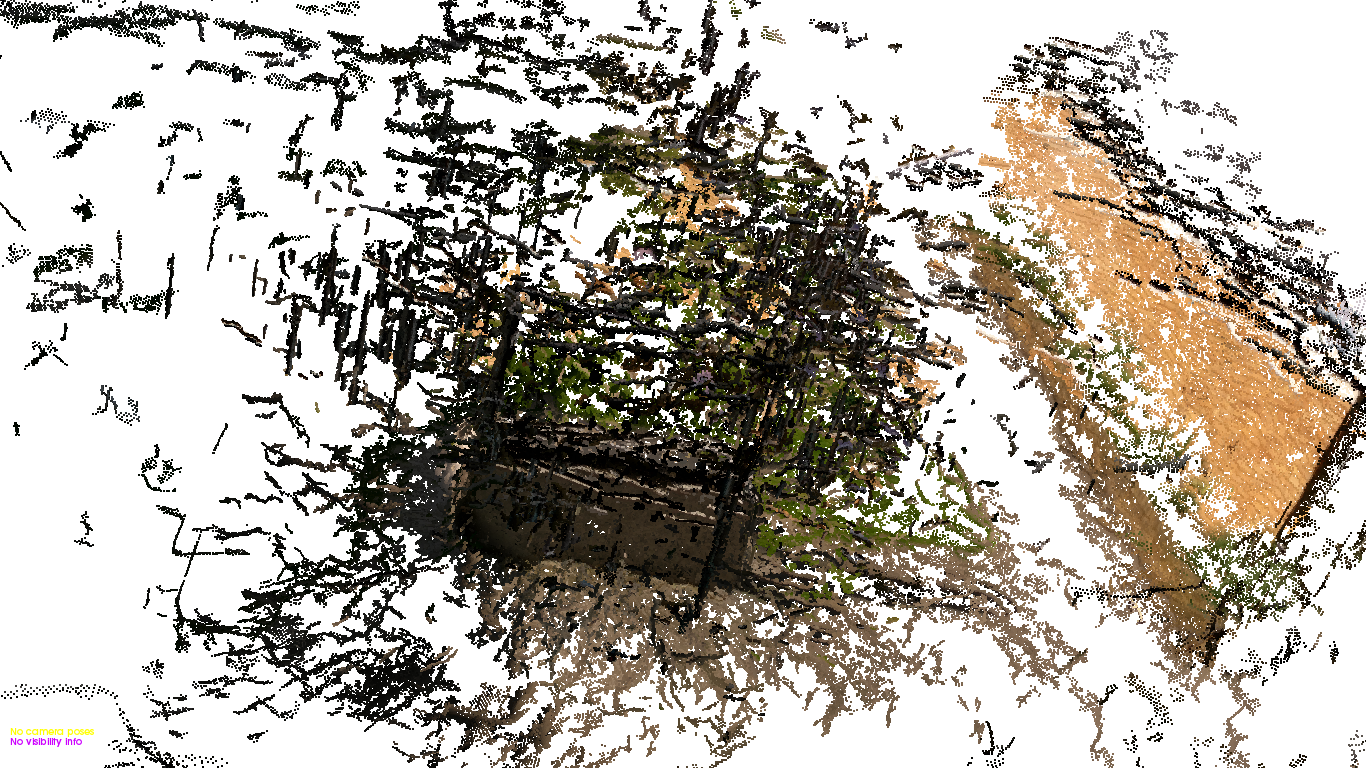
\includegraphics[width=0.9\textwidth]{img/memorial_dense}  %\label{fig:}
 }
 \caption{Good result 2: memorial dataset (cont.)}
 \label{fig:result-good2-2}
\end{figure}

\begin{figure}[htb!]
 \centering
 \subfigure[Example frame]{
  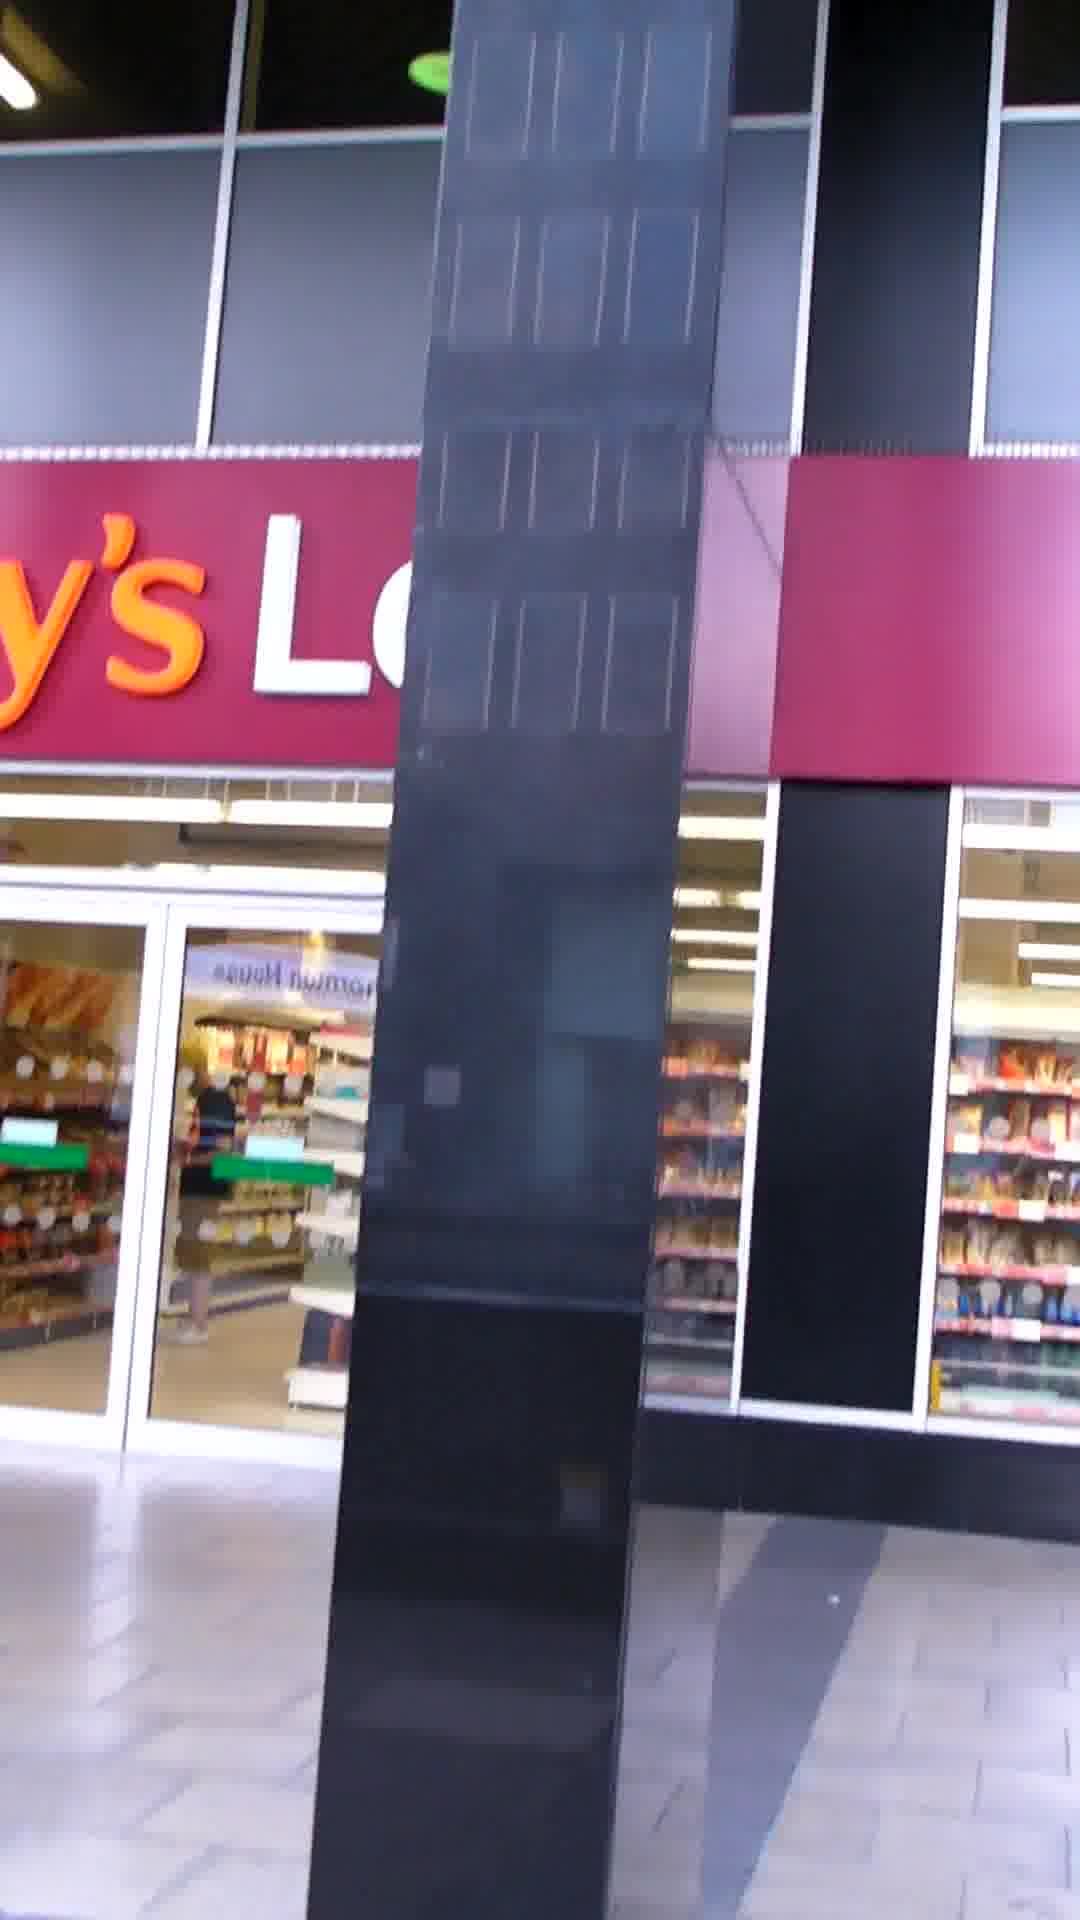
\includegraphics[width=0.25\textwidth]{img/sainsburys3_frame}  %\label{fig:}
 }
 \subfigure[Result of our Visibility-Occlusion Space Carving Veto (Alg. \ref{alg:vis-occ-carving-veto}) with $r=250, Pr_{incr}=0.001$]{
  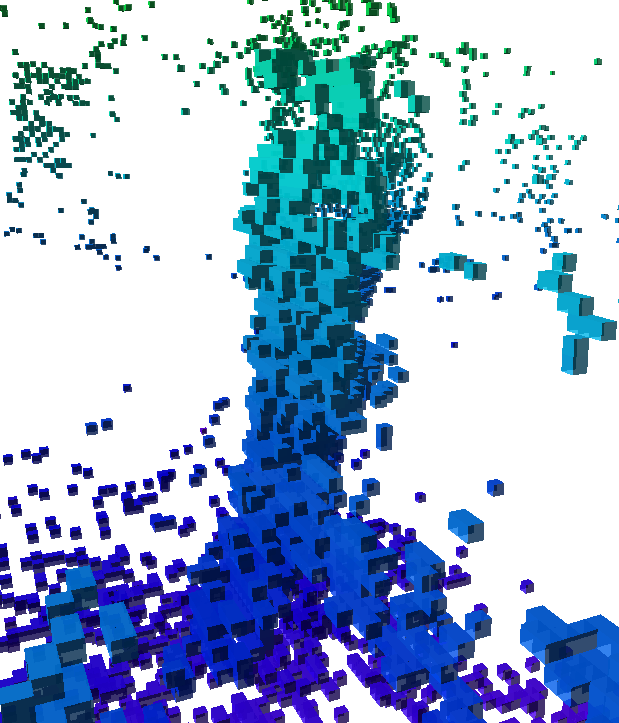
\includegraphics[width=0.40\textwidth]{img/sainsburys3_carve2}  %\label{fig:}
 }
 \subfigure[Result of CMVS/PMVS \cite{Furukawa2010}]{
  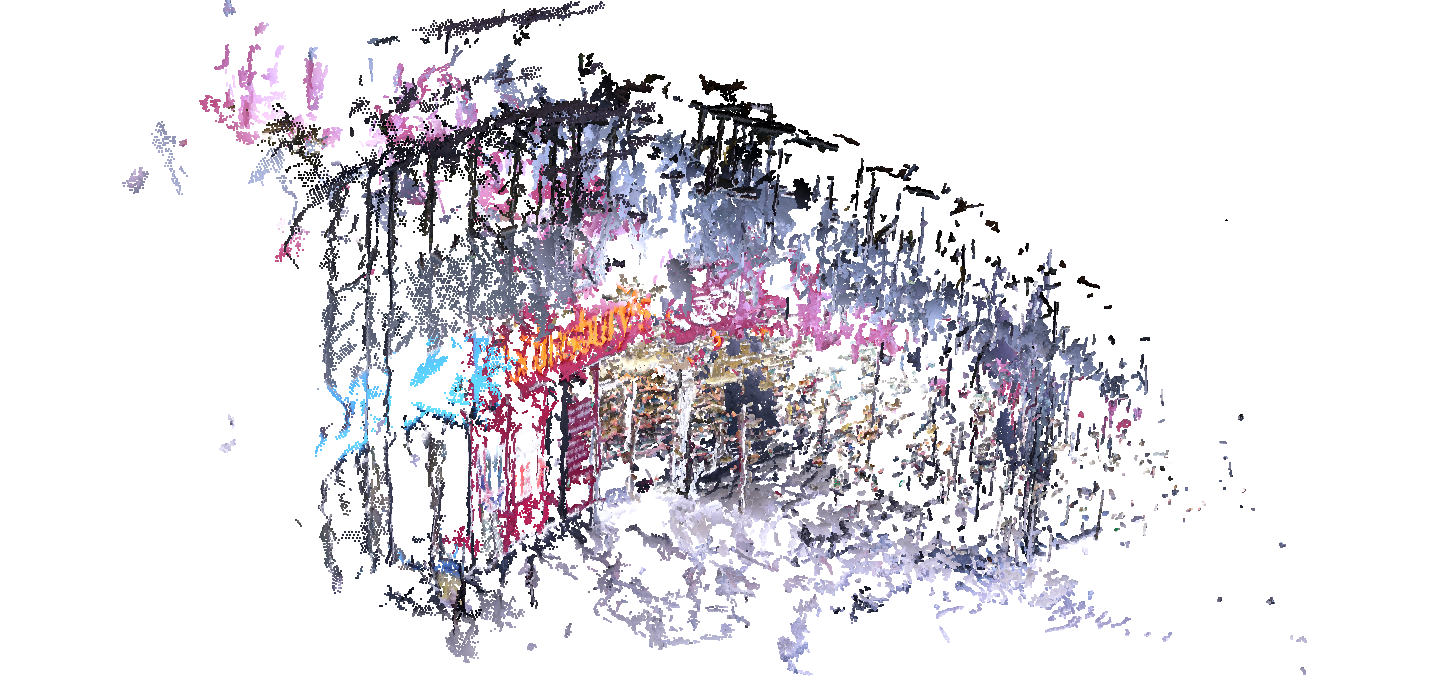
\includegraphics[width=0.9\textwidth]{img/sainsburys3_dense}  %\label{fig:}
 }
 \subfigure[Result of Photofly / 123D Catch]{
  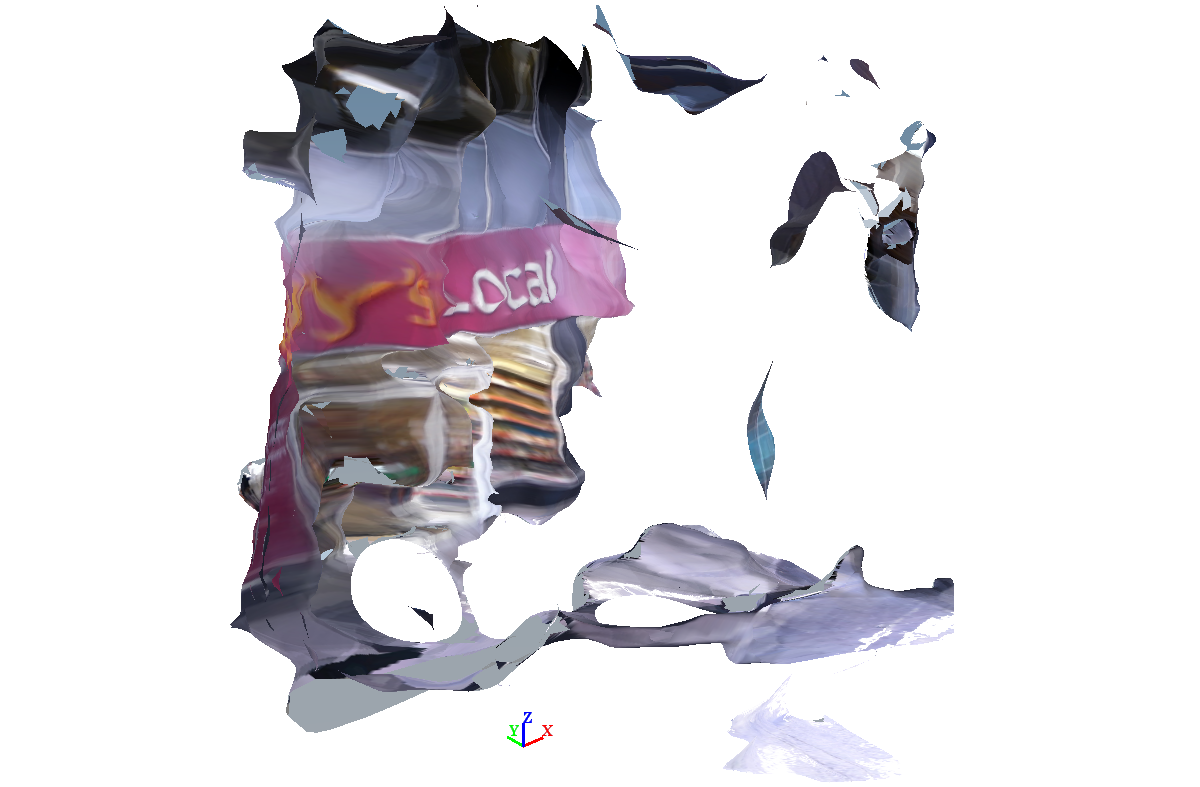
\includegraphics[width=0.9\textwidth]{img/sainsburys3_photofly}  %\label{fig:}
 }
 \caption{Comparison between our result, CMVS/PMVS \cite{Furukawa2010} result and Autodesk's closed-source Photofly / 123D Catch service for the sainsburys3 dataset (featuring a pillar of similar material as the memorial stone in Fig. \ref{fig:result-good2})}
 \label{fig:photofly}
\end{figure}


%% Evaluation
\clearpage
\section{Evaluation}
% describe results

% - review four examples
We will now discuss the examples individually, which allows us to state general observations on the tested methods. Since presenting quantitative results is difficult without ground truth, our evaluation will mostly consists of a discussion on the visual results.

Result 1 (Fig. \ref{fig:result-typical1}) consists of a sequence with poor image quality picturing two low-textured lampposts in front of a wall; nonetheless, some sparse points are reconstructed on the lampposts, probably on the edges between foreground and background. The lampposts are visible for both proposed methods and for CMVS/PMVS dense reconstruction. Visibility Space Carving causes uncarved space above and beneath the space between camera poses and the wall; although those voxels re-project inside the footage, it clearly does not have enough features on those places; however, it does show more solid structures in front of the wall. We typically found similar results for such scenes, especially when shot with a bad camera or bad lighting conditions. Usually this also means less features on feature-rich objects, decreasing the maximum resolution for which good results are obtained. The resolution settings are less important for the Visibility-Occlusion Space Carving algorithm, which marks voxels for which no information is available as unknown (thus not occupied). There, we obtain even more solid structures, but also some `clutter' caused by unstable features behind the wall, also very typical for low-quality footage with less stable background structures (\eg trees). Note that camera movement is only parallel to the wall: the maximum viewing angle causes elongated lampposts to emerge, since not enough information is present to carve space in front and behind the posts. Another key observation therefore is that enough view points needs to be provided for the algorithm if high-quality results are expected. Small low-textured objects like this are usually reasonably recovered by CMVS/PMVS.

Result 2 pictures a similar scene containing two cars and one lamppost in front of al wall. It is more challenging due to the reflective (dark) windows and sparse texture on the metal of the cars and lamppost. Indeed, sparse reconstruction does recover some but not too many points on the front objects. Visibility Space Carving again does not carve space above the wall and we had to remove some for visualisation purposes (see caption). A semi-circle has been walked, providing more views useful for finer object reconstruction. Visibility-Occlusion carving provides more solid models on higher resolution, without the need to remove clutter. CMVS/PMVS on the other hand also recovers part of the car surfaces, although holes are visible, and back and top are not recovered since they are not directly observed in enough frames. Our algorithm does recover solid models, although it may over-estimate the shape given less view points.

The third result pictures an even more challenging object with nearly no texture and some weak reflections, and people were walking in the scene while filming. Overall, the background contains less texture than a brick wall. Compared to the distance, only a short walk has been made. For Visibility Space Carving therefore low resolution has been used. Still some unwanted occupied-labelled space is floating in the air, but a solid sculpture model emerges. Visibility-Occlusion Space Carving reconstructs quite a solid structure, although some space in front of the object is labelled occupied and the object is elongated at the back (not pictured) due to views from one side only. Also compare with the \texttt{carveviewer} renderings, which should roughly correspond to what a depth map would look like (\ie single objects should have uniform colour); in the second carving result it shows a small overestimation of the shape and pictures a spike probably caused by unstable feature points at that hight. On contrary, dense reconstruction misses most of the object, and `reconstructs' quite some dirt in the air. The dirt can be caused by reflections, while the poor reconstruction of the object is likely due to low-texture.

The fourth and last full example pictures a reflective memorial stone, with little texture on it. Footage was made by walking around the object completely, obtaining many view points. Notice the good structure from motion results, even for footage of more than 800 frames; however, also observe the few wrongly triangulated feature points floating in the air around the memorial (Fig. \ref{fig:memorial_carve0}). Only part of the background, which consists of a typical urban environment, contains dense textures. Visibility Space Carving reconstructs the memorial, but leaves some holes in the model. Visibility-Occlusion Space Carving results are quite neat and can be set to high resolutions. On contrary, CMVS/PMVS performs badly on the memorial. The stone is almost invisible apart from the edges and base underneath, and the reflections cause the reconstructed scene to be filled with wrongly triangulated, non-existing small structures. Notice that the reflections are likely to cause problems on all current methods aiming at direct reconstruction (that is, methods dependent on some photo-consistency, or clean silhouettes).

Finally, the comparison in Figure \ref{fig:photofly} shows that not only CMVS/PMVS but also Autodesk's commercial geometry reconstruction system fails to reconstruct the featured reflective pillar, whereby our method does show part of the structure. It is likely that Photofly / 123D Catch will also fail on similar datasets, although no other results were returned at the time of writing.

%% discussion + limitations (data, features, parameters) -> short, keep something for conclusion
In general, low-quality footage gives reasonable results for finding small and low-textured objects, while good results can be obtained with better footage provided enough view points are captured. Therefore, the quality of the footage is somewhat relevant. Furthermore, background objects need to be present, preferably with a decent amount of texture. Unstable features, caused by moving or ambiguous objects, or bad footage, can also cause clutter to emerge. Space carving using visibility information only (Alg. \ref{alg:vis-carving}) gives reasonable results for lower resolutions. Part of the scene may remain occupied when few features are present. Visibility-Occlusion space carving, veto version (Alg. \ref{alg:vis-occ-carving-veto}) generally makes cleaner reconstructions at a higher resolution with less clutter. This is true even if objects have little texture or reflective surfaces, which cause difficulties for many existing algorithms. On the other hand, for the tested sequences CMVS/PMVS outputs high amounts of clutter for reflective objects, and surfaces of bigger low-textured objects contain holes. However, it is possible that dense stereo algorithms perform better than the proposed algorithm on general scenes containing mostly decently textured objects with Lambertian-like properties.

